% !TeX spellcheck = hr_HR-Croatian

%Prva naredba uvijek definira klasu dokumenta. Mi koristimo 'article'

\documentclass[a4paper,12pt,oneside]{article}




%***********************************************************************************
% Sada slijedi niz poziva Paketa funkcija cije ce se naredbe kasnije koristiti:
%***********************************************************************************

%Paket za upravljanje sa listama
\usepackage{enumitem}

% Paket za podesavanje brojeva stranica
\usepackage{scrlayer-scrpage}
\ifoot[]{}
\cfoot[]{}
\ofoot[\pagemark]{\pagemark}
\pagestyle{scrplain}


% Najcesce koristeni paketi za matematiku i formatiranje rada:
\usepackage{xurl}
\usepackage{url}
\usepackage{amsmath, amsthm}
\usepackage{mathtools}
\usepackage{latexsym,amsfonts,amssymb,amsbsy,graphics}
\usepackage{graphicx}
\usepackage[croatian]{babel} %Omogucava pisanje hrvatskih znakova
\usepackage{gensymb}
\usepackage{pdfpages}  %Omogucava importiranje stranica pdf fila u dokument
\usepackage{pdflscape} %Omogucava okretanje pojedine stranice landscape dok su ostale portrait


% Paket za postavke naslova i podnaslova
\usepackage{titlesec}
\newcommand{\periodafter}[1]{#1.}
\titleformat{\section}[hang]{\bf\large\uppercase}{\thesection.}{5pt}{}{}
\titleformat{\subsection}[hang]{\bf\large}{\thesubsection.}{3pt}{}{}

% Dva paketa za imenovanje slika i tablica
\usepackage{subcaption}
\usepackage[labelfont=bf,textfont=it,labelsep = colon]{caption}
\captionsetup[figure]{name=SL.}
\captionsetup[table]{name=Tab.}

% Paket sa bojama za formatiranje svega gdje se mjenja boja
\usepackage{xcolor}

% Paket za omogucavanje importiranja programskih kodova u tekst
\usepackage{listings}
\lstset{
	numbers=left,
	numberstyle=\tiny,
	columns=fullflexible,
	breaklines=true,
	postbreak=\mbox{\textcolor{red}{$\hookrightarrow$}\space},
	xleftmargin=5.0ex
}
\renewcommand{\lstlistingname}{Primjer koda}% Listing -> Algorithm

% Paket za formatiranje Sadrzaja
\usepackage[dotinlabels]{titletoc}
\dottedcontents{section}[5em]{\bfseries}{2em}{1pc}
\dottedcontents{subsection}[7em]{}{2em}{1pc}



% Najbolji paket u svemiru za matematicko pisanje tekstova
\usepackage{physics}

% Paket za postavljanje linkova na koje se moze klikat u pdfu (prema formuli broj x- click odvede na to)
\usepackage{hyperref}
\hypersetup{
	colorlinks,
	linkcolor={red!50!black},
	citecolor={blue!50!black},
	urlcolor={blue!80!black}
}


% Postavke margina stranica - NE DIRAJ

\setlength{\topmargin}{-0.7in}
\setlength{\oddsidemargin}{-2mm}
\setlength{\evensidemargin}{-2mm}
\setlength{\textwidth}{170mm}
\setlength{\textheight}{256mm}
\setlength{\parindent}{1cm}


%**************************************************************************************************************
% Prostor za tvoje pakete je ovdje:
%**************************************************************************************************************

\usepackage{tikz}
\usetikzlibrary{shapes.geometric, arrows, positioning, fit}

\emergencystretch 3em

%**************************************************************************************************************









%**************************************************************************************************************





%Kraj preamble naredbi, krece se sa pisanjem dokumenta
%**************************************************************************************************************

\begin{document}
	
	%**************************************************************************************************************
	% Postavke za numeriranje, prorede i ostalo
	%**************************************************************************************************************
	
	\setcounter{MaxMatrixCols}{20}                          %Postavka da matrica moze imati vise od 10 stupaca
	\renewcommand{\baselinestretch}{1.5}                    %postavke za prored 1.5%
	\renewcommand{\thefigure}{\thesection.\arabic{figure}}  %postavke za imenovanje slika po poglavljima%
	\renewcommand{\thetable}{\thesection.\arabic{table}}   %postavke za imenovanje tablica po poglavljima%
	\renewcommand{\theequation}{\thesection-\arabic{equation}} %postavke za brojanje jednadzbi po poglavljima%
	\renewcommand{\refname}{LITERATURA}						% Uppercase Literatura
	
	%**************************************************************************************************************
	
	
	
	
	%**************************************************************************************************************
	% NASLOVNA STRANICA
	%**************************************************************************************************************
	
	\begin{titlepage}
		
		\begin{center}{\sc\Large sveučilište josipa jurja strossmayera u osijeku}\\{\sc\Large fakultet elektrotehnike, računarstva i informacijskih tehnologija osijek}\\
			\bigskip
			
			\vspace*{2cm}
			{\large Sveučilišni diplomski studij Računarstvo}\\
			
			\vspace*{5cm}
			
			{\sc\LARGE web aplikacija za upravljanje financijskim resursima i projektima u timovima}
			
			\vspace*{1cm}
			{\large Diplomski rad}\\
			\vspace*{3cm}
			{\Large Mihael Lendvaj}\\
			\vspace*{8cm}
			{\normalsize Osijek, 2026.}
		\end{center}
		
	\end{titlepage}
	
	
	
	%**************************************************************************************************************
	% OBRASCI I FORMULARI
	%**************************************************************************************************************
	
	% Ubaciti pdf verzije D1 obrazca i izjave o originalnosti.
	
	
	%\newpage
	%\includepdf{D1_obrazac.pdf}
	%\newpage
	%\includepdf{Originalnost.pdf}
	%\newpage
	
	
	
	
	%**************************************************************************************************************
	% TABLE OF CONTENTS
	%**************************************************************************************************************
	
	{
		\hypersetup{linkcolor=black}
		\tableofcontents
	}
	%**************************************************************************************************************
	
	
	
	\newpage
	
	\section{UVOD}
	Moderno programsko inženjerstvo teži razvoju rješenja koja kombiniraju visoke performanse nativnih aplikacija i široku dostupnost klasičnih web platformi. U dinamičnim okruženjima, gdje stabilnost mrežne veze često varira, tradicionalne web aplikacije pokazuju značajne nedostatke zbog potencijalnog gubitka ili nestabilne veze sa poslužiteljem. Kao odgovor razvijen je koncept progresivnih web aplikacija (engl. \textit{Progressive Web Apps} – PWA) koji, korištenjem naprednih mehanizama poput servisnih radnika (engl. \textit{Service Workers}) i lokalnog predmemoriranja, omogućuje neometan rad aplikacije u izvanmrežnom načinu rada te naknadnu automatsku sinkronizaciju podataka.

	Glavna motivacija za razvoj sustava "Allocento" proizlazi iz potrebe za optimizacijom i osiguravanjem kontinuiteta upravljanja tokovima podataka u uvjetima nestabilne mrežne povezanosti. U klasičnim web sustavima, prekid internetske veze tijekom izvršavanja CRUD (engl. \textit{Create, Read, Update, Delete}) operacija redovito rezultira pogreškama u izvođenju i gubitkom unesenih informacija. Implementacijom PWA arhitekture unutar sustava Allocento, korisnicima se omogućuje nesmetano obavljanje poslovnih procesa i unos podataka bez obzira na trenutni status mreže, dok se složeni procesi sinkronizacije i razmjene podataka s centralnom bazom automatiziraju na razini pozadinskih servisa klijentske aplikacije.

	Pozadinski dio sustava (engl. \textit{backend}) temelji se na razvojnom okviru Laravel koji omogućuje izgradnju sigurnog i skalabilnog REST API-ja te efikasno upravljanje relacijskom bazom podataka. Prednji dio sustava (engl. \textit{frontend}) implementiran je pomoću radnog okvira Angular, čija modularna arhitektura olakšava integraciju PWA modula i upravljanje složenim stanjima aplikacije na klijentskoj strani. Vizualni identitet i konzistentnost korisničkog sučelja definirani su primjenom dizajnerskih smjernica preuzetih iz platforme Logology, čime se osigurava moderno i responzivno korisničko iskustvo.

	\subsection{Zadatak rada}
	Web aplikacija omogućuje organizacijama i timovima strukturirano praćenje i upravljanje financijskim tokovima na razini projekata i odjela. Sustav podržava evidenciju prihoda i rashoda, kategorizaciju troškova, automatsku raspodjelu sredstava po projektima te generiranje detaljnih financijskih izvještaja i analiza. Aplikacija je implementirana kao progresivna web aplikacija koristeći Angular sučelje, backend s Laravel okvirom i PostgreSQL relacijsku bazu podataka. Sustav uključuje višerazinsku autentifikaciju korisnika s definiranjem uloga i prava pristupa te podršku za ponavljajuće financijske transakcije. Projekt koristi suvremene DevOps prakse kroz GitHub Actions za kontinuiranu integraciju i automatizaciju procesa implementacije. Tema rezervirana za: Mihael Lendvaj
		

	
	
	\newpage
	\section{ANALIZA PODRUČJA I DEFINICIJA ZAHTJEVA}
		\subsection{Pregled srodnih web aplikacija}
		U današnje vrijeme na tržištu postoji velik broj aplikacija namijenjenih upravljanju financijama, proračunima i troškovima. Te se aplikacije u pravilu razlikuju prema ciljnoj skupini korisnika (osobne financije naspram poslovnih sustava), razini kompleksnosti te tehničkoj izvedbi. Kako bi se definirao položaj i opravdala potreba za sustavom "Allocento", u nastavku je pružen pregled i analiza nekoliko najznačajnijih srodnih rješenja.

		\begin{enumerate}
			\item \textbf{Splitwise} je jedna od najpopularnijih aplikacija za praćenje i raspodjelu zajedničkih troškova unutar grupa (prijatelji, cimeri, obitelj). Njezina glavna prednost leži u izuzetno jednostavnom korisničkom sučelju i automatskom izračunu tko kome duguje novac. Međutim, Splitwise je fokusiran isključivo na raspodjelu dugovanja te mu nedostaju napredne funkcionalnosti poput dugoročnog planiranja proračuna, kategorizacije prihoda i rashoda na razini cijele organizacije te praćenja projekata i odjela s definiranim budžetima.
			
			\item \textbf{Hootz} je suvremeni sustav za praćenje osobnih financija koji se ističe naprednim mogućnostima povezivanja s bankovnim računima (engl. \textit{bank syncing}) i automatskom kategorizacijom transakcija pomoću umjetne inteligencije. Aplikacija pruža izvrsnu vizualizaciju neto vrijednosti i praćenje ciljeva štednje. Unatoč tome, Hootz je dizajniran prvenstveno za pojedinačne korisnike. Nedostaje mu podrška za višekorisnički rad u stvarnom vremenu s granularnim ulogama (vlasnik, upravitelj, član) te nije prilagođen projektnom praćenju financija unutar tvrtki ili organizacija.
			
			\item \textbf{Toshl Finance} nudi bogat skup alata za ručni unos i kategorizaciju troškova, praćenje višestrukih proračuna i izradu detaljnih izvještaja. Toshl je vizualno atraktivan i podržava rad s različitim valutama. Ipak, aplikacija je u osnovi orijentirana na osobnu upotrebu, a njezin kolaborativni aspekt je minimalan. Također, aplikacija zahtijeva stalnu vezu s internetom za većinu operacija sinkronizacije te ne nudi razvijen offline-first model ponašanja na klijentskoj strani.
			
			\item \textbf{QuickBooks / Xero} predstavljaju industrijske standarde u području računovodstva i upravljanja financijama za mala i srednja poduzeća. Nude izuzetno širok spektar mogućnosti, uključujući fakturiranje, obračun poreza, upravljanje projektima i detaljne bilance. Glavni nedostatak ovih sustava je njihova visoka cijena, izrazito strma krivulja učenja te prevelika kompleksnost za timove koji trebaju samo brz, transparentan i lagan sustav za interno praćenje proračuna i projekata.
		\end{enumerate}

		Sustav "Allocento" nastoji premostiti jaz između jednostavnih alata za osobne financije (poput Toshl-a ili Hootz-a) i kompleksnih računovodstvenih sustava (poput QuickBooks-a). Allocento je dizajniran kao lagano kolaborativno rješenje koje organizacijama i timovima omogućuje praćenje financija po odjelima i projektima kroz koncept radnih prostora (engl. \textit{workspaces}), dok istovremeno rješava problem nestabilne mrežne povezanosti kroz naprednu PWA arhitekturu i offline-first pristup.
		
		\newpage
		
		\subsection{Koncept Progressive Web aplikacija}
		Progresivne web aplikacije (engl. \textit{Progressive Web Apps} – PWA) predstavljaju softversku metodologiju i skup tehnologija koje klasičnim web aplikacijama omogućuju pružanje korisničkog iskustva sličnog nativnim mobilnim ili stolnim aplikacijama. Koncept su 2015. godine osmislili Alex Russell i Frances Berriman iz tvrtke Google, s ciljem premošćivanja jaza između performansi nativnog softvera i široke dostupnosti weba.

		PWA se temelji na načelu progresivnog poboljšanja (engl. \textit{progressive enhancement}). To znači da se aplikacija ponaša kao standardna web stranica u starijim preglednicima koji ne podržavaju moderne PWA tehnologije, dok na naprednijim platformama automatski otključava dodatne mogućnosti poput rada u izvanmrežnom načinu rada, instalacije na uređaj i primanja push obavijesti.

		Ključne tehničke komponente koje čine temelj svake progresivne web aplikacije su:
		
		\begin{itemize}
			\item \textbf{Servisni radnik (engl. \textit{Service Worker}):} Skripta pisana u jeziku JavaScript koju preglednik izvršava u pozadini, odvojeno od glavne dretve korisničkog sučelja web stranice. Servisni radnik djeluje kao posrednik (engl. \textit{network proxy}) između klijentske aplikacije, mrežnih poslužitelja i lokalnog spremnika. On presreće sve mrežne zahtjeve, omogućujući implementaciju naprednih strategija predmemoriranja i potpunu funkcionalnost aplikacije bez pristupa internetu.
			
			\item \textbf{Manifest web aplikacije (engl. \textit{Web App Manifest}):} Datoteka u formatu JSON (najčešće \texttt{manifest.webmanifest} ili \texttt{manifest.json}) koja sadrži metapodatke o aplikaciji. U njoj se definiraju naziv aplikacije, ikone različitih razlučivosti, početna adresa (\textit{start URL}), boja teme te način prikaza (npr. \textit{standalone} način rada koji uklanja elemente preglednika poput adresne trake i daje aplikaciji nativni izgled).
			
			\item \textbf{Sigurnosni protokol HTTPS:} Servisni radnici posjeduju visoku razinu kontrole nad mrežnim zahtjevima i upravljanjem podacima. Zbog sprječavanja napada posredovanjem (engl. \textit{man-in-the-middle}), preglednici dopuštaju registraciju servisnih radnika isključivo preko šifriranih HTTPS veza (uz iznimku adrese \textit{localhost} tijekom lokalnog razvoja).
		\end{itemize}

		Jedan od najvećih izazova pri razvoju izvanmrežnih PWA aplikacija je odabir strategije predmemoriranja i upravljanja podacima. Dok se za statičke resurse (HTML, CSS, JavaScript datoteke, slike) koristi \textit{Cache API} koji je integriran sa servisnim radnikom, za strukturirane i transakcijske podatke (poput financijskih transakcija u sustavu Allocento) koristi se klijentska baza podataka \textbf{IndexedDB}. IndexedDB je transakcijska, NoSQL baza podataka ugrađena u preglednik, koja omogućuje pohranu velikih količina strukturiranih objekata na klijentu. Kombinacijom servisnog radnika za statičke resurse i IndexedDB-a za poslovne podatke, aplikacija postaje potpuno neovisna o trenutnom statusu mrežne veze.
		
		\newpage
		
		\subsection{Funkcionalni zahtjevi na sustav "Allocento"}
		Funkcionalni zahtjevi definiraju specifične radnje, ponašanja i usluge koje sustav mora pružiti krajnjem korisniku. Na temelju analize poslovnih potreba i službenog zadatka rada, definirani su sljedeći ključni funkcionalni zahtjevi na sustav "Allocento":
		
		\begin{itemize}
			\item \textbf{Upravljanje korisničkim računima i autentifikacija:} Sustav mora omogućiti registraciju novih korisnika, prijavu postojećih te siguran oporavak zaboravljene lozinke. Također, sustav mora podržavati verifikaciju adrese e-pošte slanjem verifikacijskih kodova na adresu korisnika.
			
			\item \textbf{Upravljanje radnim prostorima (Spaces):} Korisnik mora imati mogućnost kreiranja i sudjelovanja u više različitih radnih prostora (osobni prostori za individualne financije, kućni prostori za obiteljske potrebe i poslovni prostori za tvrtke). Sustav mora omogućiti jednostavno prebacivanje između ovih prostora bez odjave iz aplikacije.
			
			\item \textbf{Upravljanje projektima i računima (Accounts/Projects):} Unutar svakog radnog prostora korisnici moraju moći upravljati računima. U poslovnim prostorima, računi funkcioniraju kao projekti s definiranim budžetima, pri čemu sustav vizualno prikazuje omjer potrošenog i preostalog iznosa. Također, mora biti omogućeno dijeljenje pojedinog računa ili projekta s drugim radnim prostorima.
			
			\item \textbf{Evidencija i kategorizacija financijskih transakcija:} Korisnici moraju moći unositi prihode, rashode i prijenose (transfere) s jednog računa na drugi. Svaka transakcija sadrži podatke o iznosu, datumu, opisu, pripadajućoj kategoriji te projektu. Sustav mora omogućiti naknadno uređivanje i brisanje transakcija.
			
			\item \textbf{Upravljanje kategorijama troškova:} Sustav mora podržavati definiranje i upravljanje kategorijama. Administratori radnog prostora moraju imati mogućnost spajanja (\textit{merge}) dviju kategorija u jednu, pri čemu se sve povezane transakcije automatski preusmjeravaju na novu ciljnu kategoriju.
			
			\item \textbf{Kolaboracija i sustav uloga:} Korisnici moraju imati mogućnost slanja pozivnica drugim osobama za pristup određenom radnom prostoru. Sustav mora podržavati uloge (vlasnik, upravitelj, član) s definiranim pravima pristupa i modifikacije podataka.
			
			\item \textbf{Financijska analiza i izvještaji:} Sustav mora sadržavati nadzornu ploču s grafičkim prikazima (kružni i stupčasti grafikoni) raspodjele troškova po kategorijama, projektima i vremenskim razdobljima. Također, sustav mora omogućiti generiranje detaljnih filtriranih izvještaja s opcijom izvoza u PDF format.
			
			\item \textbf{Izvanmrežni način rada (Offline Mode):} U slučaju gubitka internetske veze, aplikacija mora nastaviti s radom. Korisnik mora imati mogućnost pregledavanja postojećih transakcija te unosa novih, pri čemu se sve promjene privremeno pohranjuju u lokalnu bazu podataka na uređaju.
			
			\item \textbf{Pozadinska skupna sinkronizacija (Bulk Sync):} Čim se uspostavi internetska veza, klijentska aplikacija mora automatski pokrenuti pozadinsku sinkronizaciju kako bi se svi lokalno uneseni podaci u jednom paketu (engl. \textit{bulk}) poslali na poslužitelj i spremili u centralnu bazu podataka.
			
			\item \textbf{Web Push obavijesti:} Sustav mora omogućiti primanje obavijesti u stvarnom vremenu (npr. kada korisnik primi pozivnicu za novi radni prostor), čak i kada aplikacija nije aktivno otvorena u pregledniku.
		\end{itemize}
		
		\subsection{Nefunkcionalni zahtjevi na sustav "Allocento"}
		Nefunkcionalni zahtjevi definiraju atribute kvalitete, tehnička ograničenja te standarde koje sustav mora zadovoljiti kako bi osigurao optimalan rad, sigurnost i dobro korisničko iskustvo. Definirani su sljedeći nefunkcionalni zahtjevi na sustav:
		
		\begin{itemize}
			\item \textbf{Performanse i brzina odziva:} Aplikacija se mora učitavati brzo, čak i na uređajima s lošijom internetskom vezom. Vrijeme odziva REST API-ja za osnovne CRUD operacije ne bi smjelo prelaziti nekoliko stotina milisekundi.
			
			\item \textbf{Responzivnost i dizajn sučelja:} Korisničko sučelje mora biti u potpunosti responzivno, prilagođeno ekranima svih veličina (od pametnih telefona do stolnih računala). Vizualni identitet mora biti konzistentan, ugodan i profesionalan, prateći dizajnerske smjernice definirane kroz sustav Logology.
			
			\item \textbf{Pouzdanost i integritet podataka:} Gubitak mrežne veze tijekom unosa podataka ne smije dovesti do gubitka unesenih informacija ili rušenja aplikacije. Lokalne baze podataka na klijentu moraju osigurati transakcijski integritet prije sinkronizacije s glavnom bazom.
			
			\item \textbf{Sigurnost i privatnost:} Sva komunikacija između klijenta i poslužitelja mora biti šifrirana primjenom HTTPS protokola. Pristup API-ju mora biti zaštićen tokenima (Laravel Sanctum), a podaci različitih radnih prostora moraju biti strogo izolirani na razini baze podataka i autorizacijskih middleware-a.
			
			\item \textbf{Jednostavnost instalacije i prenosivost:} Budući da se radi o PWA aplikaciji, instalacija na uređaj mora biti omogućena izravno iz preglednika jednim klikom, bez potrebe za preuzimanjem preko službenih trgovina aplikacijama (App Store, Google Play). Aplikacija mora raditi na svim modernim preglednicima (Chrome, Safari, Firefox, Edge).
		\end{itemize}
	
	
	\newpage
	\section{TEHNOLOGIJE, ALATI I RAZVOJNO OKRUŽENJE}
		\subsection{Tehnologije na strani poslužitelja}
		Razvoj pozadinskog dijela (engl. \textit{backend}) sustava "Allocento" zahtijevao je odabir tehnološkog stoga koji omogućuje brzu izgradnju sigurnog, skalabilnog i performantnog REST API-ja. Za tu svrhu odabran je jezik PHP te radni okvir Laravel, u kombinaciji sa sustavom za autentifikaciju Laravel Sanctum.

		\textbf{PHP} (engl. \textit{Hypertext Preprocessor}) je široko rasprostranjeni skriptni jezik opće namjene koji se izvršava na strani poslužitelja te je primarno dizajniran za razvoj web aplikacija. Moderni PHP (inačica 8 i novije) donosi značajna poboljšanja u performansama, strogo tipiziranje podataka te podršku za moderne objektno-orijentirane paradigme, što ga čini izuzetno prikladnim za razvoj složenih poslovnih sustava.
		
		\textbf{Laravel} je besplatni radni okvir (engl. \textit{framework}) otvorenog koda namijenjen razvoju web aplikacija u jeziku PHP prema arhitektonskom obrascu MVC (model-pogled-kontroler). Laravel se ističe elegantnom sintaksom i bogatim ekosustavom koji nudi rješenja za uobičajene zadatke u web razvoju, kao što su:
		\begin{itemize}
			\item \textbf{Eloquent ORM:} Objektno-relacijsko mapiranje koje omogućuje interakciju s bazom podataka putem objektno-orijentirane sintakse umjesto pisanja sirovih SQL upita.
			
			\item \textbf{Sustav migracija:} Omogućuje kontrolu verzija baze podataka i jednostavno dijeljenje sheme baze među članovima tima.
			
			\item \textbf{Laravel Queues:} Sustav redova čekanja za asinkronu obradu vremenski zahtjevnih zadataka (npr. slanje e-pošte ili obrada ponavljajućih transakcija).
			
			\item \textbf{Middleware slojevi:} Filtri koji presreću HTTP zahtjeve i omogućuju kontrolu pristupa, validaciju radnih prostora i sigurnosne provjere.
		\end{itemize}

		\textbf{Laravel Sanctum} pruža jednostavan i siguran sustav za autentifikaciju jednostraničnih web aplikacija (engl. \textit{Single Page Applications} – SPA) i mobilnih aplikacija. U sustavu Allocento, Sanctum se koristi za autentifikaciju klijenta izdavanjem API tokena (engl. \textit{API tokens}) nakon uspješne prijave korisnika. Ti se tokeni pohranjuju na klijentskoj strani te šalju u zaglavlju svakog HTTP zahtjeva (\texttt{Authorization: Bearer token}), omogućujući siguran pristup zaštićenim API rutama.

		\textbf{REST API} (engl. \textit{Representational State Transfer}) predstavlja arhitektonski stil za razvoj distribuiranih hipermedijskih sustava. API u sustavu Allocento temelji se na principima REST-a, što podrazumijeva upotrebu standardnih HTTP metoda (GET za dohvaćanje, POST za kreiranje, PUT za ažuriranje i DELETE za brisanje resursa) i razmjenu podataka isključivo u strukturiranom formatu JSON (engl. \textit{JavaScript Object Notation}).

		\newpage

		\subsection{Tehnologije na strani klijenta}
		Klijentski dio (engl. \textit{frontend}) sustava Allocento razvijen je kao progresivna web aplikacija pomoću razvojnog okvira Angular, jezika TypeScript te tehnologija za lokalnu pohranu i konfiguraciju PWA značajki.

		\textbf{Angular} je klijentski radni okvir otvorenog koda temeljen na jeziku TypeScript, kojeg razvija i održava tvrtka Google. Angular se odlikuje modularnom arhitekturom i prikladan je za izgradnju robusnih jednostraničnih web aplikacija (SPA). U razvoju sustava Allocento korištene su moderne značajke Angulara:
		\begin{itemize}
			\item \textbf{Samostalne komponente (engl. \textit{Standalone Components}):} Pojednostavljuju strukturu projekta eliminirajući potrebu za klasičnim modulima (\texttt{NgModule}), čime se smanjuje količina popratnog koda (engl. \textit{boilerplate}) i ubrzava učitavanje.
			
			\item \textbf{Angular Signals (Signali):} Novi reaktivni model uveden u Angular koji omogućuje granularno upravljanje stanjem aplikacije. Signali prate promjene vrijednosti u stvarnom vremenu i automatski ažuriraju isključivo one dijelove korisničkog sučelja koji izravno ovise o toj vrijednosti, što značajno poboljšava performanse renderiranja u usporedbi s tradicionalnim sustavom provjere promjena (engl. \textit{change detection}).
		\end{itemize}

		\textbf{TypeScript} je programski jezik otvorenog koda koji predstavlja strogo tipizirani nadskup (engl. \textit{superset}) jezika JavaScript. Svi TypeScript programi prevode se u običan JavaScript kako bi se mogli izvršavati u bilo kojem pregledniku. Glavne prednosti TypeScripta su statička provjera tipova, poboljšana podrška u razvojnim okruženjima (automatsko dovršavanje koda, refaktoriranje) te bolja čitljivost i održivost koda u većim projektima.

		\textbf{IndexedDB i prilagođeni LocalDbService:} IndexedDB je klijentski NoSQL sustav baze podataka ugrađena u preglednik, namijenjen pohrani strukturiranih podataka. Za razliku od \textit{LocalStoragea} koji ima ograničen kapacitet i sinkronu izvedbu, IndexedDB radi asinkrono i podržava transakcije. U sustavu Allocento, za lakše upravljanje ovim asinkronim operacijama razvijena je namjenska klijentska klasa \textbf{LocalDbService}, koja omata nativne IndexedDB pozive i transakcije u JavaScript obećanja (engl. \textit{Promises}). Ovaj servis se koristi za privremeno spremanje transakcija kada je uređaj izvan mreže te za lokalno predmemoriranje podataka.

		\textbf{Angular Service Worker (ngsw):} Za konfiguraciju PWA funkcionalnosti korišten je službeni Angularov paket \texttt{@angular/service-worker}. On automatski generira servisnog radnika na temelju konfiguracijske datoteke \texttt{ngsw-config.json}, upravlja lokalnim predmemoriranjem statičkih resursa (HTML, CSS, JavaScript datoteke, ikone) te omogućuje integraciju s preglednikovim sustavom za primanje pozadinskih obavijesti (engl. \textit{Web Push Notifications}) putem servisa \texttt{SwPush}.

		\subsection{Alat za definiciju vizualnog identiteta i brenda aplikacije}
		Za definiranje dizajnerskih smjernica, logotipa, tipografije i palete boja korištena je platforma \textbf{Logology}. Logology je specijalizirani alat za automatizirano brendiranje i kreiranje vizualnog identiteta softverskih proizvoda. 
		
		Na temelju dizajnerskog profila sustava Allocento, odabrana je paleta boja s naglašenim tamnim i svijetlim tonovima te specifični fontovi (Space Mono i Outfit). Ove su smjernice potom prenesene u razvojni sustav klijentske aplikacije u obliku globalnih CSS varijabli (engl. \textit{CSS custom properties}), čime se postigla vizualna konzistentnost, responzivnost i moderan izgled sučelja (engl. \textit{premium UX}).

		\subsection{Sustav za upravljanje relacijskim bazama podataka i web poslužitelj}
		Upravljanje podacima na strani poslužitelja organizirano je kroz kombinaciju dvaju relacijskih sustava za upravljanje bazama podataka (SUBP) ovisno o okruženju, dok je za posluživanje aplikacije odabran Nginx.

		\textbf{SQLite} je lagana, ugrađena relacijska baza podataka otvorenog koda koja ne zahtijeva zasebni poslužiteljski proces jer se cijela baza pohranjuje u jednu datoteku na disku. U sustavu Allocento, SQLite se koristi isključivo u razvojnom okruženju (engl. \textit{development environment}) zbog jednostavnosti postavljanja, nultog konfiguracijskog napora i brzine izvršavanja testova.

		\textbf{PostgreSQL} je napredni objektno-relacijski sustav upravljanja bazom podataka poznat po pouzdanosti, robusnosti i usklađenosti s ACID standardima. PostgreSQL se koristi u produkcijskom okruženju sustava Allocento, gdje osigurava visoku razinu performansi pri konkurentnom pristupu bazi podataka od strane više različitih korisnika, podržava napredne indeksacije te omogućuje sigurno skaliranje sustava.

		\textbf{Nginx} je visokoperformantni web poslužitelj s asinkronom arhitekturom upravljanom događajima (engl. \textit{event-driven architecture}). U ovom projektu Nginx ima ulogu obrnutog proxyja (engl. \textit{reverse proxy}) koji zaprima sve klijentske HTTP zahtjeve, statički poslužuje izgrađenu Angular frontend aplikaciju, a zahtjeve namijenjene API-ju prosljeđuje PHP-FPM procesu Laravel backend aplikacije. Nginx je također konfiguriran za usmjeravanje svih SPA ruta prema početnoj \texttt{index.html} datoteci Angulara.

		\subsection{DevOps alati i sustavi za upravljanje verzijama koda}
		Kontinuirana integracija i isporuka (CI/CD), kao i suradnja na razvoju programskog koda, ostvareni su primjenom sustava Git, platforme GitHub te GitHub Actions servisa.

		\textbf{Git} je distribuirani sustav kontrole verzija koji prati promjene u izvornom kodu tijekom razvoja softvera. Omogućuje grananje koda (engl. \textit{branching}) za neovisan razvoj pojedinih značajki i njihovo naknadno spajanje (engl. \textit{merging}).

		\textbf{GitHub} je internetska usluga za udomljavanje repozitorija projekata koja koristi Git. GitHub služi kao centralno mjesto za pohranu koda sustava Allocento te olakšava timski rad i pregled koda (engl. \textit{code review}).
		
		\textbf{GitHub Actions} je platforma za automatizaciju procesa razvoja softvera koja se pokreće na GitHubovim poslužiteljima. U ovom projektu postavljen je automatizirani radni tijek (engl. \textit{workflow}) u datoteci \texttt{deploy.yml}. On se pokreće automatski prilikom svakog guranja (engl. \textit{push}) novog koda na glavnu granu. Radni tijek provodi prevođenje klijentske aplikacije (\texttt{npm run build:prod}), provjerava sintaksu i ispravnost backend koda, a zatim automatski prebacuje izgrađene datoteke na produkcijski poslužitelj, čime se osigurava brza, pouzdana i automatizirana isporuka softvera.
	
	
	\newpage
	\section{ARHITEKTURA I DIZAJN SUSTAVA}
		\subsection{Konceptualna arhitektura}
		Sustav "Allocento" temelji se na klijent-poslužitelj (engl. \textit{client-server}) arhitekturi s jasnim razdvajanjem odgovornosti. Klijentski dio aplikacije razvijen je kao jednostranična progresivna web aplikacija (PWA), dok pozadinski dio funkcionira kao beskontaktni (engl. \textit{stateless}) REST API.
		
		PWA koncept donosi specifičnu konceptualnu arhitekturu u kojoj klijentska aplikacija ne komunicira izravno s mrežom, već se sve mrežne interakcije presreću na razini preglednika pomoću servisnog radnika (\textit{Service Worker}). Servisni radnik djeluje kao posrednik i upravlja lokalnim predmemoriranjem statičkih resursa.
		
		Kada je uređaj spojen na internet (engl. \textit{online} način rada), servisni radnik propušta HTTP zahtjeve API-ja kroz mrežni poslužitelj Nginx do Laravel backend aplikacije. Laravel komunicira s glavnom PostgreSQL bazom podataka te vraća podatke klijentu u formatu JSON.
		
		U izvanmrežnom (engl. \textit{offline}) načinu rada, servisni radnik preusmjerava klijenta na lokalno predmemorirane statičke resurse (HTML, CSS, JS), dok se transakcijski podaci dohvaćaju i spremaju unutar klijentske baze podataka IndexedDB. Čim se internetska veza ponovno uspostavi, klijentska aplikacija pokreće asinkroni pozadinski posao koji skupno sinkronizira sve promjene s glavnim poslužiteljem.

		\begin{figure}[h!]
			\centering
			\begin{tikzpicture}[node distance=2.2cm, auto]
				% Styles
				\tikzstyle{block} = [draw, fill=blue!10, rectangle, minimum height=2.5em, minimum width=8.5em, rounded corners, align=center, font=\small]
				\tikzstyle{sw} = [draw, fill=orange!10, rectangle, minimum height=2.5em, minimum width=9.5em, rounded corners, align=center, font=\small]
				\tikzstyle{storage} = [draw, fill=yellow!15, rectangle, minimum height=2.5em, minimum width=8.5em, rounded corners, align=center, font=\small]
				\tikzstyle{server} = [draw, fill=purple!10, rectangle, minimum height=2.5em, minimum width=8.5em, rounded corners, align=center, font=\small]
				\tikzstyle{db} = [draw, fill=green!10, rectangle, minimum height=2.5em, minimum width=8.5em, rounded corners, align=center, font=\small]
				\tikzstyle{arrow} = [thick,->,>=stealth]

				% Nodes
				\node (browser) [block] {Klijentski preglednik \\ (Korisnik)};
				\node (sw) [sw, right=of browser, xshift=0.8cm] {Service Worker \\ (Mrežni posrednik)};
				\node (cache) [storage, below=of sw, yshift=-0.3cm] {Lokalna baza \\ (IndexedDB / Cache)};
				\node (nginx) [block, right=of sw, xshift=0.8cm] {Nginx poslužitelj \\ (Obrnuti proxy)};
				\node (laravel) [server, below=of nginx, yshift=-0.3cm] {Laravel backend \\ (REST API)};
				\node (db) [db, below=of laravel, yshift=-0.3cm] {PostgreSQL \\ (Glavna baza)};

				% Connections
				\draw [arrow] (browser) -- node {Zahtjev} (sw);
				\draw [arrow] (sw) -- node [right] {Offline / Cache} (cache);
				\draw [arrow] (sw) -- node {Mreža} (nginx);
				\draw [arrow] (nginx) -- (laravel);
				\draw [arrow] (laravel) -- (db);
				
			\end{tikzpicture}
			\caption{Konceptualna arhitektura sustava Allocento i tokovi podataka}
			\label{fig:konceptualna_arhitektura}
		\end{figure}
		
		\newpage

		\subsection{Arhitektura klijentskog dijela}
		Klijentska aplikacija u Angularu strukturirana je kroz tri osnovna sloja, čime se postiže labava povezanost (engl. \textit{loose coupling}) i visoka održivost koda:
		\begin{enumerate}
			\item \textbf{UI sloj (Stranice i komponente):} Odgovoran je za prikazivanje korisničkog sučelja i prikupljanje korisničkih akcija. Korištenjem Angular signala (\textit{Signals}) ostvaruje se reaktivno povezivanje podataka (engl. \textit{data binding}) s predlošcima (HTML), bez potrebe za stalnim ručnim osvježavanjem komponenti.
			
			\item \textbf{Servisni sloj (Business Logic):} Sadrži globalne servise koji upravljaju zajedničkim stanjima aplikacije (npr. trenutno aktivni radni prostor, odabir jezika, status mrežne povezanosti, upravljanje push obavijestima). Servisi služe kao most između UI sloja i repozitorija.
			
			\item \textbf{Sloj repozitorija (Data Access Layer - DAL):} Repozitoriji (poput \texttt{TransactionRepository} ili \texttt{AccountRepository}) predstavljaju apstrakciju pristupa podacima. U ovom sloju se provodi logika offline rada: repozitorij provjerava status mreže te odlučuje hoće li upit proslijediti API servisu (koji koristi HTTP klijent) ili lokalnom repozitoriju (koji izravno komunicira s IndexedDB bazom podataka).
		\end{enumerate}

		\begin{figure}[h!]
			\centering
			\begin{tikzpicture}[node distance=1.5cm, auto]
				% Styles
				\tikzstyle{comp} = [draw, fill=blue!10, rectangle, minimum height=2.5em, minimum width=9.5em, rounded corners, align=center, font=\small]
				\tikzstyle{serv} = [draw, fill=orange!10, rectangle, minimum height=2.5em, minimum width=9.5em, rounded corners, align=center, font=\small]
				\tikzstyle{repo} = [draw, fill=purple!10, rectangle, minimum height=2.5em, minimum width=9.5em, rounded corners, align=center, font=\small]
				\tikzstyle{storage} = [draw, fill=yellow!15, rectangle, minimum height=2.5em, minimum width=9.5em, rounded corners, align=center, font=\small]
				\tikzstyle{arrow} = [thick,->,>=stealth]

				% Nodes
				\node (ui) [comp] {Angular UI sloj \\ (Stranice i komponente)};
				\node (services) [serv, below=of ui] {Angular servisi \\ (Sync, Auth, Signals)};
				\node (repos) [repo, below=of services] {Repozitoriji \\ (DAL apstrakcija)};
				\node (localdb) [storage, below=of repos, xshift=-2.6cm] {Lokalna pohrana \\ (IndexedDB / LocalDb)};
				\node (http) [comp, below=of repos, xshift=2.6cm, fill=gray!10] {HttpClient \\ (REST API)};

				% Connections
				\draw [arrow] (ui) -- node {Signals} (services);
				\draw [arrow] (services) -- (repos);
				\draw [arrow] (repos) -- node [left] {Offline} (localdb);
				\draw [arrow] (repos) -- node [right] {Online} (http);
				
			\end{tikzpicture}
			\caption{Arhitekturni slojevi klijentskog dijela u Angularu}
			\label{fig:klijentska_arhitektura}
		\end{figure}
		
		\newpage

		\subsection{Arhitektura poslužiteljskog dijela}
		Arhitektura poslužiteljskog dijela u Laravelu strukturirana je tako da podržava višekorisnički rad na razini radnih prostora (\textit{multi-tenancy}). Slojevi se mogu podijeliti na:
		\begin{itemize}
			\item \textbf{Sloj ruta i Middleware-a:} Zaprimljeni zahtjevi prolaze kroz Sanctum autentifikaciju, nakon čega se primjenjuje specifični \texttt{workspace} middleware. On provjerava zaglavlje \texttt{X-Workspace-Id} i osigurava da prijavljeni korisnik ima prava pristupa tom radnom prostoru te ga postavlja u kontekst zahtjeva.
			
			\item \textbf{Kontroleri (Controllers):} Odgovorni su za validaciju unesenih podataka iz HTTP zahtjeva, pozivanje odgovarajućih servisa poslovne logike te oblikovanje i vraćanje odgovora u formatu JSON.
			
			\item \textbf{Servisni sloj (Services):} Sadrži čistu poslovnu logiku aplikacije. Kontroleri prosljeđuju zahtjeve servisima koji provode složenije operacije (npr. spajanje kategorija, provjera budžeta, generiranje izvještaja) i time sprječavaju gomilanje logike u kontrolerima (koncept \textit{fat models, thin controllers} ili \textit{service layer pattern}).
			
			\item \textbf{Eloquent ORM Modeli:} Predstavljaju tablice u bazi podataka i definiraju veze među entitetima.
		\end{itemize}

		\begin{figure}[h!]
			\centering
			\begin{tikzpicture}[node distance=1.2cm, auto]
				% Styles
				\tikzstyle{box} = [draw, fill=purple!10, rectangle, minimum height=2.2em, minimum width=12em, rounded corners, align=center, font=\small]
				\tikzstyle{db} = [draw, fill=green!10, rectangle, minimum height=2.2em, minimum width=12em, rounded corners, align=center, font=\small]
				\tikzstyle{arrow} = [thick,->,>=stealth]

				% Nodes
				\node (route) [box] {Rute i Workspace Middleware};
				\node (controller) [box, below=of route] {API Kontroleri \\ (Validacija zahtjeva)};
				\node (service) [box, below=of controller] {Poslovni servisi \\ (Servisni sloj)};
				\node (model) [box, below=of service] {Eloquent ORM Modeli \\ (Modeli baze podataka)};
				\node (db) [db, below=of model] {Relacijska baza podataka \\ (PostgreSQL / SQLite)};

				% Connections
				\draw [arrow] (route) -- (controller);
				\draw [arrow] (controller) -- (service);
				\draw [arrow] (service) -- (model);
				\draw [arrow] (model) -- (db);
				
			\end{tikzpicture}
			\caption{Slojevita arhitektura poslužiteljskog dijela u Laravelu}
			\label{fig:posluziteljska_arhitektura}
		\end{figure}
		
		\newpage

		\subsection{Model baze podataka}
		Baza podataka je relacijskog karaktera i dizajnirana je tako da podržava rad s različitim valutama, višestrukim prostorima i granularnim pravima pristupa. Ključni entiteti i njihove relacije su:
		
		\begin{itemize}
			\item \textbf{Korisnik (\texttt{users}):} Sadrži osnovne podatke o korisniku (ime, e-mail, lozinka, fotografija profilna, aktivni radni prostor). Korisnik može kreirati više radnih prostora te sudjelovati u prostorima drugih korisnika.
			
			\item \textbf{Radni prostor (\texttt{workspaces}):} Predstavlja izolirani financijski prostor (osobni, obiteljski, poslovni). Svi ostali entiteti (računi, kategorije, transakcije) vezani su uz određeni radni prostor.
			
			\item \textbf{ (Pivot tablica):} Povezuje korisnike i radne prostore u odnosu više-prema-više (N:M). Sadrži atribut uloge (\textit{role}) koji može biti \textit{owner} (vlasnik), \textit{manager} (upravitelj) ili \textit{member} (član), te status pozivnice (\textit{pending}, \textit{accepted}).
			
			\item \textbf{Račun / Projekt (\texttt{accounts}):} Predstavlja financijski račun koji pripada radnom prostoru. Sadrži naziv, valutu, vrstu, trenutno stanje (\textit{balance}) i početni budžet (\textit{opening\_balance}). U poslovnim prostorima ovi računi predstavljaju projekte i njihove proračune.
			
			\item \textbf{Kategorija (\texttt{categories}):} Definira kategoriju troška ili prihoda. Kategorije mogu biti globalne (sistemske) ili lokalne (vezane uz radni prostor). Podržano je hijerarhijsko povezivanje preko polja \texttt{parent\_id} (kategorije i podkategorije).
			
			\item \textbf{Transakcija (\texttt{transactions}):} Predstavlja osnovni zapis o financijskom toku. Povezana je s računom, kategorijom i korisnikom koji ju je unio. Sadrži tip (prihod, rashod, transfer), iznos, datum i opis.
			
			\item \textbf{RecurringTemplate (\texttt{recurring\_templates}):} Pohranjuje predloške za transakcije koje se automatski ponavljaju u određenim vremenskim intervalima (npr. mjesečno plaćanje režija).
		\end{itemize}

		\begin{figure}[h!]
			\centering
			\begin{tikzpicture}[auto]
				% Styles
				\tikzstyle{entity} = [draw, fill=blue!10, rectangle, minimum height=2.2em, minimum width=8.5em, align=center, font=\small\bfseries, rounded corners=2pt]
				\tikzstyle{arrow} = [thick,->,>=stealth]

				% Nodes with absolute coordinates (planar layout)
				\node (user) [entity] at (0, 5.5) {User};
				\node (member) [entity] at (4.2, 4.5) {WorkspaceUser \\ (Pivot N:M)};
				\node (workspace) [entity] at (0, 3.5) {Workspace};
				\node (account) [entity] at (-2.8, 1.5) {Account \\ (Project)};
				\node (category) [entity] at (2.8, 1.5) {Category};
				\node (transaction) [entity] at (0, -0.5) {Transaction};

				% Connections
				\draw [arrow] (user) -- node [left, font=\tiny] {1:N} (workspace);
				\draw [arrow] (user) -- node [above right, font=\tiny] {1:N} (member);
				\draw [arrow] (workspace) -- node [below right, font=\tiny] {1:N} (member);
				\draw [arrow] (workspace) -- node [above left, font=\tiny] {1:N} (account);
				\draw [arrow] (workspace) -- node [above right, font=\tiny] {1:N} (category);
				\draw [arrow] (account) -- node [below left, font=\tiny] {1:N} (transaction);
				\draw [arrow] (category) -- node [below right, font=\tiny] {1:N} (transaction);

			\end{tikzpicture}
			\caption{Pojednostavljeni ER dijagram baze podataka sustava Allocento}
			\label{fig:er_dijagram}
		\end{figure}
	
	
	\newpage
	\section{IMPLEMENTACIJA SUSTAVA "ALLOCENTO"}
		\subsection{Implementacija REST API-ja i upravljanje tokovima podataka}
		Pozadinski dio sustava Allocento razvijen je kao usluga REST API koja klijentu pruža pristup resursima baze podataka na temelju sigurnih i standardiziranih protokola komunikacije. 

		Autentifikacija korisnika temelji se na tokenima i ostvarena je primjenom paketa \textbf{Laravel Sanctum}. Kada se korisnik registrira ili prijavi, poslužitelj generira jedinstveni token i vraća ga klijentu. Klijent sprema token u lokalnu pohranu te ga prilaže u zaglavlju svakog sljedećeg zahtjeva (\texttt{Authorization: Bearer token}). Rute API-ja koje zahtijevaju prijavu zaštićene su ugrađenim middleware-om \texttt{auth:sanctum} koji provjerava valjanost tokena prije nego što dopusti izvršavanje kontrolera.

		Ključni aspekt implementacije API-ja u sustavu Allocento je osiguravanje izolacije radnih prostora (engl. \textit{workspace scoping}). Budući da korisnici mogu sudjelovati u više radnih prostora (osobni, kućni, poslovni), sustav mora jamčiti da korisnik može čitati ili mijenjati samo one podatke koji pripadaju trenutno aktivnom prostoru. U tu svrhu razvijen je prilagođeni posrednički sloj \textbf{WorkspaceMiddleware}.
		
		Ovaj middleware presreće svaki HTTP zahtjev namijenjen zaštićenim rutama. On iz zaglavlja zahtjeva dohvaća parametar \texttt{X-Workspace-Id}. Potom provjerava nalazi li se taj radni prostor u bazi podataka te ima li prijavljeni korisnik ulogu (članstvo) u njemu. Ako su provjere uspješne, middleware učitava objekt radnog prostora iz baze podataka i sprema ga izravno u atribute zahtjeva pod ključem \texttt{\_workspace}. To omogućuje kontrolerima da odmah pristupe podacima aktivnog prostora putem poziva \texttt{\$request->get('\_workspace')}, bez potrebe za ponavljanjem upita i provjera prava pristupa.

		Validacija podataka provodi se na razini kontrolera prije bilo kakvog unosa ili izmjene u bazi podataka. Laravel omogućuje strogu validaciju tipova podataka, formata datuma i provjeru postojanja stranih ključeva u povezanim tablicama (npr. provjera postoji li \texttt{category\_id} ili \texttt{project\_id} u bazi). U slučaju neuspjele validacije, sustav automatski odbija zahtjev i vraća odgovor s HTTP statusom \texttt{422 Unprocessable Entity} i opisom pogreške, dok se uspješne operacije potvrđuju odgovarajućim statusima (npr. \texttt{201 Created} za uspješan unos transakcije ili \texttt{204 No Content} za brisanje).

		\newpage
		
		\subsection{Primjena vizualnog identiteta}
		Dizajnerske smjernice i vizualni identitet sustava Allocento definirani su pomoću platforme Logology, s ciljem stvaranja modernog, čistog i prepoznatljivog korisničkog sučelja koje pruža premium korisničko iskustvo.

		Integracija vizualnog identiteta u programski kod klijentskog dijela aplikacije ostvarena je definiranjem dizajnerskog sustava (engl. \textit{design system tokens}) unutar globalne CSS datoteke. U pseudo-klasi \texttt{:root} definirane su klijentske CSS varijable (engl. \textit{CSS custom properties}) koje predstavljaju temeljne dizajnerske atribute aplikacije:
		\begin{itemize}
			\item \textbf{Paleta boja:} Definirane su varijable za primarnu i sekundarnu pozadinu, tekst, obrube te brendirane naglašene boje, poput ljubičaste (\texttt{--color-}\allowbreak\texttt{brand-}\allowbreak\texttt{purple} sa specifičnom heksadecimalnom vrijednošću \texttt{\#7f5af0} preuzetom iz Logology smjernica) i zelene (\texttt{--color-}\allowbreak\texttt{brand-}\allowbreak\texttt{green} vrijednosti \texttt{\#2cb67d}).
			
			\item \textbf{Tipografija:} Za strukturiranje tekstualnih elemenata definirana su dva osnovna fonta. Font \textit{Outfit} koristi se za većinu elemenata korisničkog sučelja (naslove, izbornike, opise) jer osigurava visoku čitljivost i moderan izgled. Font \textit{Space Mono} (monospace font) koristi se za prikaz brojčanih vrijednosti, transakcija i tablica, što pridonosi prepoznatljivom tehničkom i strukturiranom izgledu financijskog sustava.
			
			\item \textbf{Oblikovanje sučelja:} Definirane su standardizirane vrijednosti za zaobljenost rubova kartica i gumba (npr. \texttt{--border-radius-lg: 12px}) te razmake među elementima, čime se postiže vizualna konzistentnost na svim stranicama.
		\end{itemize}

		Korištenjem ovih varijabli kroz sintaksu \texttt{var(--ime-varijable)} u CSS datotekama Angular komponenti, postignuta je visoka fleksibilnost koda. Ovaj pristup omogućuje jednostavno održavanje vizualnog identiteta, brze promjene tema i prilagodbu sučelja različitim uređajima.

		\newpage

		\subsection{Strukturiranje klijentskih komponenti i upravljanje stanjima}
		Klijentski dio aplikacije u Angularu strukturiran je korištenjem modernog pristupa samostalnih komponenti (engl. \textit{standalone components}), čime je uklonjena potreba za tradicionalnim modulima. Svaka komponenta je neovisna cjelina koja u svom dekoratoru eksplicitno definira svoje ovisnosti (druge komponente, direktive ili cijevi).
		
		Usmjeravanje (engl. \textit{routing}) u aplikaciji definirano je u datoteci \texttt{app.routes.ts}. Za optimizaciju performansi učitavanja primijenjeno je lijeno učitavanje (engl. \textit{lazy loading}) putem funkcije \texttt{loadComponent}. To znači da preglednik preuzima programski kod za specifične stranice (npr. nadzornu ploču, izvještaje ili postavke) tek kada korisnik klikne na njih, čime se drastično smanjuje veličina početnog paketa aplikacije i ubrzava prvo učitavanje.

		Upravljanje stanjem aplikacije i reaktivnost sučelja u potpunosti su implementirani pomoću **Angular Signala** (engl. \textit{Angular Signals}), novog reaktivnog primitiva koji donosi finu kontrolu nad promjenama stanja. U sustavu Allocento signali se koriste za:
		\begin{itemize}
			\item \textbf{Praćenje aktivnog konteksta:} Servis \texttt{WorkspaceService} izlaže signal \texttt{activeWorkspace =} \allowbreak \texttt{signal<Workspace} \allowbreak \texttt{| null>(null)}. Kada se korisnik prebaci u drugi radni prostor, vrijednost signala se ažurira, a sve komponente koje ovise o tom signalu automatski se i trenutačno ponovno iscrtavaju s novim podacima.
			
			\item \textbf{Dinamičko filtriranje transakcija:} Korištenjem izvedenih signala (\texttt{computed}) ostvareno je filtriranje popisa transakcija na klijentu u stvarnom vremenu. Primjerice, signal \texttt{filteredTransactions} automatski ponovno izračunava filtrirani popis transakcija čim se promijeni bilo koji od ulaznih signala filtara (npr. odabrani datum početka, projekt ili kategorija). Budući da se koristi \texttt{computed}, izračun se provodi samo kada se promijene stvarni podaci, a rezultati se predmemoriraju.
			
			\item \textbf{Sinkronizaciju izvanmrežnih operacija:} Reaktivni signali se koriste i za praćenje broja transakcija koje čekaju u lokalnom redu za sinkronizaciju, omogućujući trenutačni prikaz indikatora izvanmrežnog rada korisniku.
		\end{itemize}
		
		\newpage
		
		
		\subsection{Konfiguracija PWA funkcionalnosti i servisnih radnika}
		Razvoj progresivne web aplikacije zahtijeva konfiguriranje servisnog radnika koji upravlja predmemoriranjem statičkih resursa kako bi aplikacija bila dostupna u izvanmrežnom načinu rada. U klijentskom dijelu sustava Allocento, ova se konfiguracija nalazi unutar datoteke \texttt{ngsw-config.json}.

		Konfiguracijska datoteka definira pravila predmemoriranja podijeljena u dvije glavne skupine:
		\begin{enumerate}
			\item \textbf{Grupe resursa (engl. \textit{assetGroups}):} Odnose se na statičke datoteke aplikacije. Podijeljene su na:
			\begin{itemize}
				\item \textit{Core resursi (App):} HTML, CSS i JavaScript datoteke potrebne za pokretanje same aplikacije. Za njih je odabrana strategija \texttt{prefetch}, što znači da se preuzimaju i spremaju u lokalni spremnik odmah prilikom prvog učitavanja aplikacije.
				
				\item \textit{Sporedni resursi (Assets):} Slike, ikone i vanjski fontovi. Za njih se koristi strategija \texttt{lazy}, odnosno učitavaju se i spremaju u spremnik tek kada ih aplikacija prvi put zatraži.
			\end{itemize}
			
			\item \textbf{Grupe podataka (engl. \textit{dataGroups}):} Odnose se na dinamičke API zahtjeve. Za rute poput popisa transakcija ili nadzorne ploče konfigurirana je strategija \texttt{freshness} (mreža ima prioritet, a u slučaju nedostupnosti poslužitelja koristi se lokalno predmemorirani odgovor) s definiranim maksimalnim vijekom trajanja (\texttt{maxAge}) i maksimalnim brojem spremljenih odgovora (\texttt{maxSize}).
		\end{enumerate}

		\subsubsection{Integracija i konfiguracija Web Push obavijesti}
		Poticajne obavijesti (engl. \textit{Web Push Notifications}) omogućuju poslužitelju slanje informacija klijentu čak i kada aplikacija nije aktivna u pregledniku. Implementacija ovog sustava u Allocentu koristi Push API i Notification API standarde te se temelji na tri entiteta: klijentskom pregledniku, posredničkom Push servisu preglednika i Laravel poslužitelju aplikacije.

		Za osiguravanje privatnosti i autentičnosti pošiljatelja koristi se protokol **VAPID** (engl. \textit{Voluntary Application Server Identification}). Na poslužitelju se generira par ključeva: javni i privatni VAPID ključ.
		
		Tijek registracije i slanja obavijesti odvija se na sljedeći način:
		\begin{enumerate}
			\item Klijentska aplikacija u Angularu, koristeći servis \texttt{SwPush}, traži privolu korisnika za primanje obavijesti. Ako korisnik odobri, preglednik šalje zahtjev Push servisu (koji održava proizvođač preglednika, npr. Google za Chrome ili Apple za Safari) prilažući javni VAPID ključ.
			
			\item Push servis generira jedinstveni objekt pretplate (engl. \textit{subscription object}) koji sadrži jedinstvenu adresu (\textit{endpoint}) i ključeve za enkripciju podataka (\textit{p256dh} i \textit{auth}).
			
			\item Angular aplikacija šalje taj objekt pretplate na Laravel backend putem rute \texttt{POST /api/push/subscribe}, gdje se pretplata sprema u bazu podataka i povezuje s autentificiranim korisnikom.
			
			\item Kada na poslužitelju nastupi događaj (npr. slanje pozivnice za radni prostor), Laravel pokreće pozadinski posao koji uz pomoć privatnog VAPID ključa kriptira poruku i šalje je na adresu definiranu u objektu pretplate. Push servis prima poruku, prepoznaje uređaj i isporučuje je pregledniku koji pokreće servisnog radnika u pozadini kako bi prikazao vizualnu obavijest korisniku.
		\end{enumerate}

		\subsubsection{Sinkronizacija podataka u izvanmrežnom načinu rada (Bulk Sync)}
		Jedan od najvećih izazova pri razvoju sustava Allocento bio je osiguravanje konzistentnosti podataka i kontinuiranog rada u izvanmrežnom načinu rada. Rješenje je implementirano kombinacijom klijentske IndexedDB baze podataka (putem prilagođenog servisa \texttt{LocalDbService}), upravljanjem lokalnim stanjima i jedinstvenim endpointom za skupnu sinkronizaciju na backendu.

		Kada korisnik izvrši CRUD operaciju (npr. unos nove transakcije) dok je uređaj offline, proces se odvija kroz sljedeće korake:
		\begin{enumerate}
			\item \textbf{Generiranje lokalnog identiteta:} Budući da se baza na poslužitelju ne može kontaktirati za dodjelu primarnog ključa (ID), klijentski repozitorij generira privremeni negativni ID na temelju trenutne vremenske oznake (npr. \texttt{-1719504500000}). Negativni ID osigurava da se lokalno kreirani zapisi odmah razlikuju od onih koji su potvrđeni u glavnoj bazi podataka.
			
			\item \textbf{Lokalno spremanje i prikaz:} Transakcija se odmah sprema u klijentsku IndexedDB tablicu \texttt{transactions} i reaktivno prikazuje u korisničkom sučelju, pružajući korisniku osjećaj da aplikacija radi bez zastoja.
			
			\item \textbf{Dodavanje u red čekanja:} Istodobno se u tablicu \texttt{offline\_queue} dodaje objekt akcije koji opisuje operaciju (npr. \texttt{\{action: 'create', payload: \{...\}, local\_id: -1719504500000\}} ili \texttt{\{action: 'delete', transaction\_id: 15\}}).
		\end{enumerate}

		Kada se mrežna veza uspostavi (što klijent detektira putem osluškivača \texttt{window.online}), aktivira se servis \texttt{SyncService} koji pokreće metodu \texttt{syncOfflineQueue()}:
		\begin{enumerate}
			\item Servis učitava sve zapise iz tablice \texttt{offline\_queue}.
			
			\item Grupirane operacije se pakiraju u jedno polje (\textit{operations}) i šalju na poslužitelj u samo jednom HTTP zahtjevu putem rute \texttt{POST /api/transactions/sync}.
			
			\item Poslužitelj otvara bazu podataka unutar transakcije (\texttt{DB::transaction}) kako bi se osigurala atomarnost (ako jedna operacija ne uspije, cijeli se paket vraća na prethodno stanje). Laravel prolazi kroz operacije redom:
			\begin{itemize}
				\item Za operaciju \texttt{create}, stvara se zapis u bazi podataka i generira stvarni ID. Ako je poslan \texttt{local\_id}, poslužitelj bilježi mapiranje (npr. \texttt{-1719504500000 => 345}).
				
				\item Za operacije \texttt{update} ili \texttt{delete}, ako se one odnose na novoosnovanu transakciju (koja ima negativni ID), poslužitelj koristi mapiranu vrijednost stvarnog ID-ja kako bi proveo izmjenu u bazi podataka.
			\end{itemize}
			
			\item Poslužitelj vraća odgovor s mapiranim ID-jevima i statusom sinkronizacije. Klijent ažurira IndexedDB s pravim ID-jevima i briše uspješno sinkronizirane zapise iz tablice \texttt{offline\_queue}.
		\end{enumerate}
		
		\newpage

		\subsection{Prikaz ključnih segmenata programskog koda}
		U nastavku su prikazani ključni segmenti programskog koda koji ilustriraju rješenja opisana u ovom poglavlju. Primjer koda \ref{lst:resolve_workspace} prikazuje implementaciju middleware-a u Laravelu koji razrješava radni prostor na temelju zaglavlja HTTP zahtjeva i postavlja ga u kontekst aplikacije.

\begin{lstlisting}[language=PHP, caption={Laravel middleware za razrjeđivanje aktivnog radnog prostora}, label={lst:resolve_workspace}]
class ResolveWorkspace
{
    public function handle(Request $request, Closure $next): Response
    {
        $user = $request->user();
        if (!$user) {
            return $next($request);
        }

        $workspaceId = $request->header('X-Workspace-ID');
        $workspace = null;

        if ($workspaceId) {
            $workspace = $user->workspaces()->where('workspaces.id', $workspaceId)->first();
        }

        if (!$workspace) {
            $workspaceId = $user->favorite_workspace_id;
            if ($workspaceId) {
                $workspace = $user->workspaces()->where('workspaces.id', $workspaceId)->first();
            }
        }

        if (!$workspace) {
            $workspace = $user->workspaces()->first();
            if ($workspace) {
                $user->update(['favorite_workspace_id' => $workspace->id]);
            } else {
                return response()->json(['error' => 'No workspace context available.'], 400);
            }
        }

        $request->merge(['_workspace' => $workspace]);
        $request->attributes->set('workspace', $workspace);

        return $next($request);
    }
}
\end{lstlisting}


\newpage

		Primjer koda \ref{lst:angular_create} ilustrira metodu u Angular repozitoriju \texttt{TransactionRepository} koja detektira offline način rada, stvara privremenu transakciju s negativnim ID-jem, sprema je lokalno radi trenutačnog prikaza u sučelju i dodaje je u red čekanja za naknadnu sinkronizaciju.

\begin{lstlisting}[language=Java, caption={Klijentsko kreiranje transakcije i pohrana u offline red čekanja}, label={lst:angular_create}]
create(accountId: number, payload: Partial<Transaction>): Observable<Transaction> {
  if (!this.appInitializer.isOnlineMode) {
    const localId = -Date.now(); // Negativni ID za offline zapise
    const localTx: Transaction = {
      id: localId,
      accountId: accountId,
      type: payload.type || 'expense',
      amount: payload.amount || 0,
      date: payload.date || new Date().toISOString(),
      description: payload.description || null,
      categoryId: payload.categoryId || null,
      projectId: payload.projectId || null,
      targetAccountId: payload.targetAccountId || null,
      excludeFromAnalytics: payload.excludeFromAnalytics || null,
      user: null
    };

    return from(
      (async () => {
        await this.localDb.put('transactions', this.mapTransactionToLocal(localTx));
        const queueItem = {
          action: 'create',
          payload: {
            account_id: accountId,
            type: localTx.type,
            amount: localTx.amount,
            date: localTx.date,
            description: localTx.description,
            category_id: localTx.categoryId,
            project_id: localTx.projectId,
            target_account_id: localTx.targetAccountId,
            exclude_from_analytics: localTx.excludeFromAnalytics,
            local_id: localId
          }
        };
        await this.localDb.put('offline_queue', queueItem);
        return localTx;
      })()
    );
  }
  
  
  return this.api.post<any>(`/accounts/${accountId}/transactions`, payload).pipe(
    map(api => this.mapApiToTransaction(api)),
    tap(async (tx) => {
      await this.localDb.put('transactions', this.mapTransactionToLocal(tx));
    })
  );
}
\end{lstlisting}


		Primjer koda \ref{lst:laravel_sync} prikazuje metodu \texttt{sync} u Laravel kontroleru \texttt{TransactionController} koja prima skupni paket operacija, izvršava ih unutar jedne transakcije baze podataka i mapira privremene ID-jeve.

\begin{lstlisting}[language=PHP, caption={Laravel kontroler za skupnu sinkronizaciju i mapiranje ID-jeva}, label={lst:laravel_sync}]
public function sync(Request $request): JsonResponse
{
    $workspace = $request->get('_workspace');
    $accountIds = $workspace->accounts()->pluck('accounts.id')->toArray();

    $data = $request->validate([
        'operations' => ['required', 'array', 'max:500'],
        'operations.*.action' => ['required', 'in:create,update,delete'],
        'operations.*.transaction_id' => ['nullable', 'integer'],
        'operations.*.payload' => ['nullable', 'array'],
    ]);

    $results = DB::transaction(function () use ($data, $request, $accountIds) {
        $syncedCount = 0;
        $errors = [];
        $idMappings = []; // Karta: negativni ID => stvarni ID iz baze

        foreach ($data['operations'] as $index => $operation) {
            $action = $operation['action'];
            $payload = $operation['payload'] ?? [];
            $transactionId = $operation['transaction_id'] ?? null;
            
            // Mapiranje ako je transakcija stvorena offline u istom paketu
            if (in_array($action, ['update', 'delete']) && $transactionId < 0 && isset($idMappings[$transactionId])) {
                $transactionId = $idMappings[$transactionId];
            }

            try {
                if ($action === 'create') {
                    $accountId = $payload['account_id'] ?? null;
                    if (!$accountId || !in_array($accountId, $accountIds)) {
                        throw new \Exception('Access denied or account not found.');
                    }
                    $tx = $this->transactionService->createForAccount($request->user(), $accountId, $payload);
                    if (isset($payload['local_id']) && $payload['local_id'] < 0) {
                        $idMappings[$payload['local_id']] = $tx->id;
                    }
                    $syncedCount++;
                } elseif ($action === 'update') {
                    $transaction = Transaction::where('id', $transactionId)->whereIn('account_id', $accountIds)->first();
                    if (!$transaction) throw new \Exception('Transaction not found.');
                    $this->transactionService->updateForAccount($request->user(), $transaction->account_id, $transactionId, $payload);
                    $syncedCount++;
                } elseif ($action === 'delete') {
                    $transaction = Transaction::where('id', $transactionId)->whereIn('account_id', $accountIds)->first();
                    if ($transaction) {
                        $this->transactionService->deleteForAccount($request->user(), $transaction->account_id, $transactionId);
                        $syncedCount++;
                    }
                }
            } catch (\Exception $e) {
                $errors[] = [
                    'index' => $index,
                    'error' => $e->getMessage()
                ];
            }
        }
        return ['synced' => $syncedCount, 'errors' => $errors, 'id_mappings' => $idMappings];
    });

    return response()->json($results, count($results['errors']) > 0 ? 207 : 200);
}
\end{lstlisting}

		\subsection{Automatizacija implementacije aplikacije (CI/CD cjevovod)}
		Uvođenje suvremenih DevOps praksi osigurano je pisanjem CI/CD cjevovoda (engl. \textit{CI/CD pipeline}) pomoću platforme GitHub Actions. Datoteka \texttt{deploy.yml} definira automatizirani proces isporuke koda na produkcijski poslužitelj čim se promjene spoje (engl. \textit{merge}) na glavnu granu (\texttt{main}) repozitorija.
		
		Cjevovod se sastoji od jednog posla (\textit{job}) pod nazivom \texttt{deploy} koji se izvodi u virtualnom okruženju \texttt{ubuntu-latest}. Radni tijek provodi sljedeće faze:
		\begin{enumerate}
			\item \textbf{Preuzimanje koda (Checkout):} Koristi se akcija \texttt{actions/checkout} za preuzimanje izvornog koda iz Git repozitorija u radni prostor radnika.
			
			\item \textbf{Uspostava SSH veze:} Pokreće se SSH agent i učitava se privatni SSH ključ pohranjen u sigurnim postavkama repozitorija (\textit{GitHub Secrets}). Time se omogućuje sigurna komunikacija s produkcijskim poslužiteljem bez izlaganja lozinki.
			
			\item \textbf{Sinkronizacija koda na poslužitelju:} Putem SSH naredbi na udaljenom poslužitelju povlače se najnovije promjene iz repozitorija na produkcijsku lokaciju.
			
			\item \textbf{Izgradnja pozadinskog dijela (Backend build):} Automatski se ažurira produkcijska konfiguracijska datoteka \texttt{.env} s postavkama PostgreSQL baze podataka i VAPID ključevima. Zatim se pokreće instalacija PHP ovisnosti (\texttt{composer install}) i primjenjuju se migracije baze podataka (\texttt{php artisan migrate}) kako bi se shema baze uskladila s kodom.
			
			\item \textbf{Izgradnja klijentskog dijela (Frontend build):} Na poslužitelju se instaliraju klijentske ovisnosti pomoću naredbe \texttt{npm ci} te se prevodi klijentska Angular aplikacija u produkcijski paket naredbom \texttt{npm run build:prod}. Izgrađeni statički resursi smještaju se u direktorij poslužitelja kojeg Nginx koristi za posluživanje weba.
		\end{enumerate}

		Ovakav cjevovod smanjuje mogućnost ljudske pogreške pri ručnom prijenosu datoteka na poslužitelj i osigurava da je na produkciji uvijek aktivna verzija koda koja je uspješno prošla provjere.
	
	
	\newpage
	\section{KORISNIČKO SUČELJE I PRIKAZ RADA APLIKACIJE}
		U ovom poglavlju prikazan je praktični rad i vizualni izgled aplikacije Allocento kroz ključne korisničke tokove. Prikazi zaslona (engl. \textit{screenshots}) demonstriraju primjenu definiranog vizualnog identiteta i responzivnog dizajna prilagođenog različitim rezolucijama (računala i mobilnih uređaja).

		\subsection{Autentifikacija, autorizacija i upravljanje ulogama u timu}
		Prvi korak u korištenju aplikacije Allocento je autentifikacija korisnika. Korisničko sučelje za prijavu i registraciju oblikovano je s fokusom na jednostavnost i preglednost, u skladu s brendiranim bojama.

		Stranica za registraciju zahtijeva unos imena, e-mail adrese i lozinke. Nakon slanja podataka, Laravel backend šalje verifikacijski e-mail s poveznicom za potvrdu računa. Dok e-mail nije verificiran, klijentska aplikacija onemogućuje pristup glavnim financijskim funkcijama i prikazuje obavijest o potrebi verifikacije. Prijava se vrši unosom e-mail adrese i lozinke, nakon čega se generira Sanctum token koji klijent sprema u lokalnu pohranu te se korisnik preusmjerava na nadzornu ploču. Prikaz sučelja za autentifikaciju prikazan je na slici \ref{fig:login-registration}.

		\begin{figure}[h!]
			\centering
			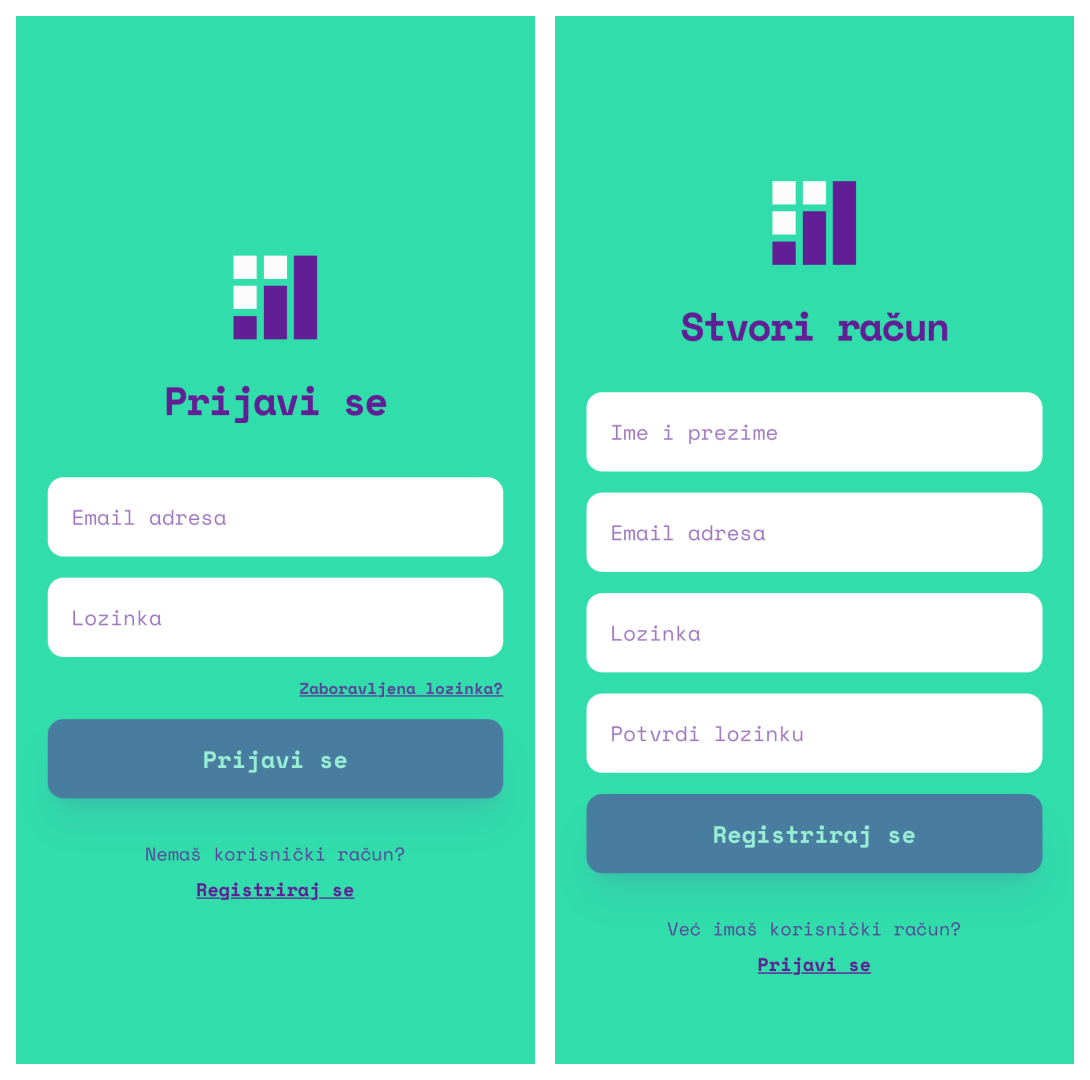
\includegraphics[width=0.8\textwidth]{assets/login_registration.png}
			\caption{Sučelje za prijavu i registraciju korisnika}
			\label{fig:login-registration}
		\end{figure}

		Nakon uspješne prijave, korisnik može kreirati novi radni prostor (engl. \textit{workspace}) ili se prebaciti u neki od postojećih u kojima je član. Prilikom kreiranja prostora korisnik odabire tip prostora: osobni (engl. \textit{personal}) ili timski/poslovni (engl. \textit{company}). 

		U timskim radnim prostorima dostupna je kartica za upravljanje članovima tima. Vlasnik radnog prostora može pozvati nove članove upisivanjem njihove e-mail adrese. Sustav šalje pozivnicu koja se prikazuje pozvanom korisniku pri njegovom sljedećem ulasku u aplikaciju. Korisnik pozivnicu može prihvatiti ili odbiti. Unutar radnog prostora podržane su tri uloge s različitim razinama autorizacije:
		\begin{itemize}
			\item \textbf{Vlasnik (Owner):} Korisnik koji je kreirao radni prostor. Ima puna prava upravljanja računima, kategorijama, projektima, članovima tima i ulogama te može obrisati radni prostor.
			
			\item \textbf{Član (Member):} Može unositi, mijenjati i brisati transakcije, pregledavati analitiku i izvještaje te dodavati nove kategorije i projekte. Ne može upravljati članovima tima niti brisati radni prostor.
			
			\item \textbf{Gledatelj (Viewer):} Ima isključivo prava čitanja (engl. \textit{read-only}). Može pregledavati nadzornu ploču, izvještaje i popise transakcija, ali ne može unositi nove podatke niti raditi bilo kakve izmjene.
		\end{itemize}
		Sučelje za kreiranje radnog prostora i slanje pozivnica prikazano je na slici \ref{fig:workspace-settings}.

		\begin{figure}[h!]
			\centering
			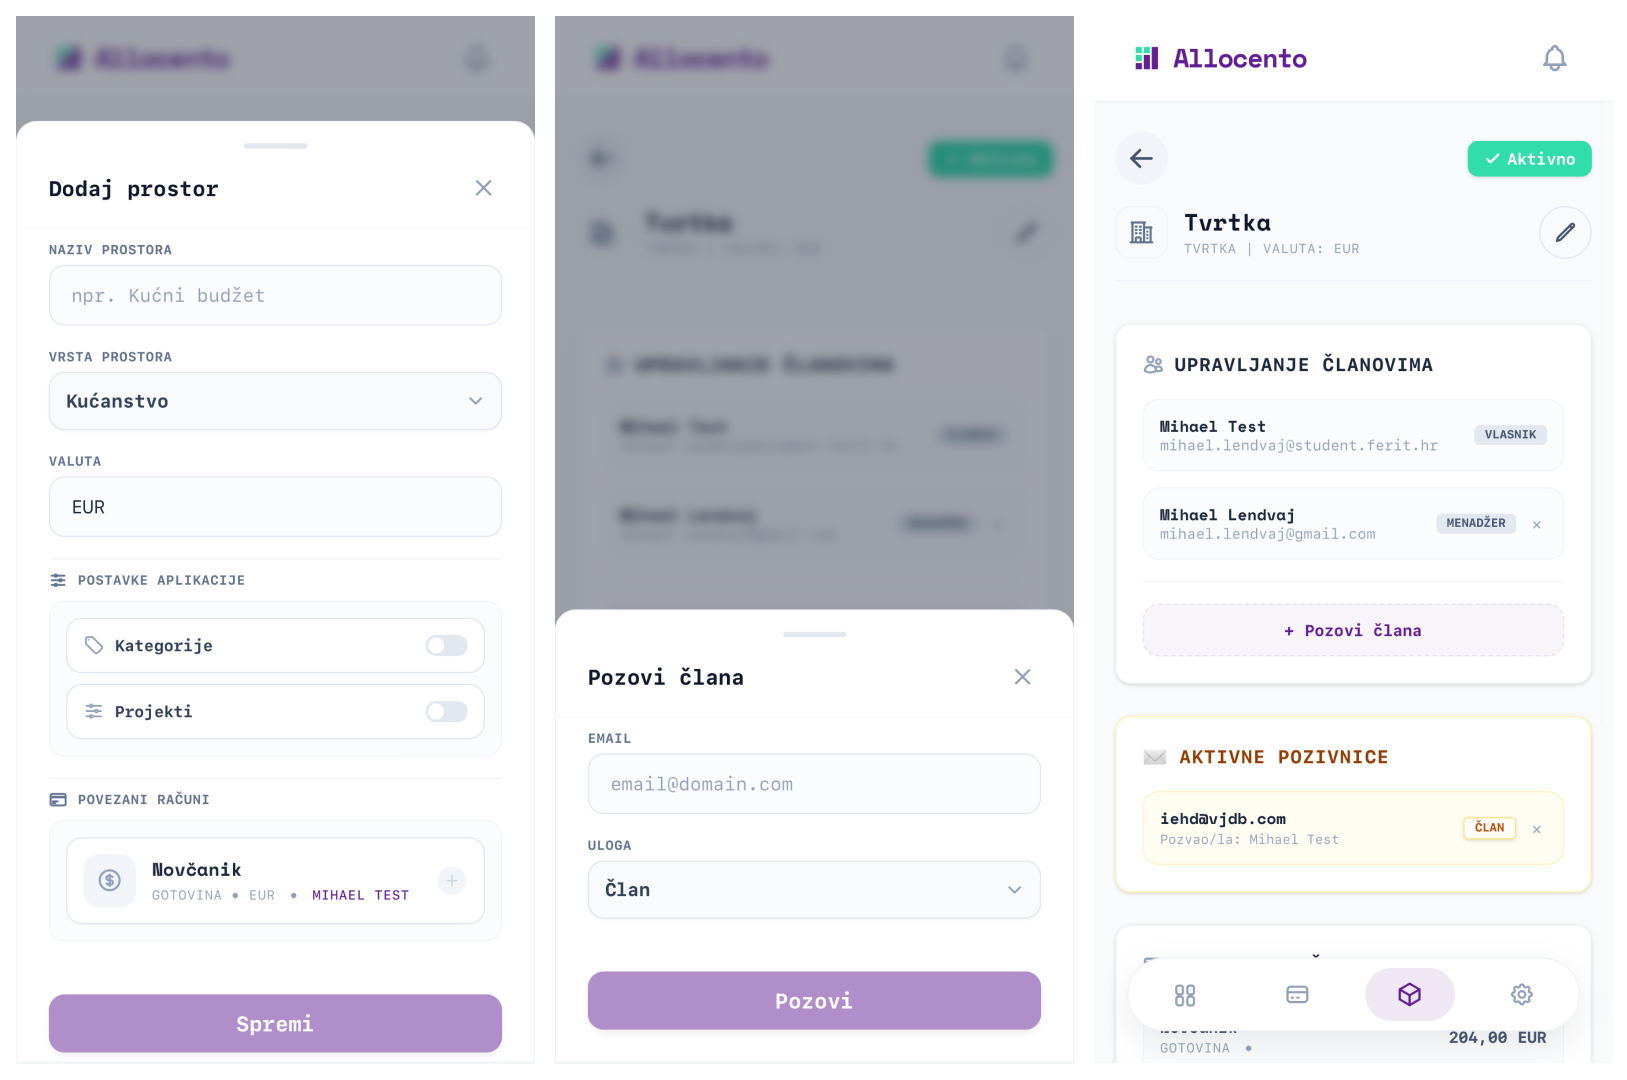
\includegraphics[width=0.8\textwidth]{assets/workspace_settings.png}
			\caption{Upravljanje radnim prostorima i pozivanjem članova tima}
			\label{fig:workspace-settings}
		\end{figure}
		
		\newpage

		\subsection{Glavna nadzorna ploča, analitika i financijski izvještaji}
		Glavna nadzorna ploča (engl. \textit{Dashboard}) predstavlja središnje mjesto aplikacije na kojem korisnik dobiva trenutačni uvid u financijsko stanje odabranog radnog prostora. 
		
		Sučelje nadzorne ploče sastoji se od sljedećih cjelina:
		\begin{itemize}
			\item \textbf{Izbornik radnog prostora u zaglavlju:} Omogućuje brzi prijelaz iz jednog radnog prostora u drugi, pri čemu se svi podaci na zaslonu reaktivno ažuriraju bez osvježavanja stranice.
			
			\item \textbf{Ukupni saldo (Balance):} Zbroj svih raspoloživih sredstava na računima unutar aktivnog radnog prostora. Ispod salda nalazi se brza akcija za dodavanje nove transakcije.
			
			\item \textbf{Prikaz projektnih budžeta:} Kod poslovnih radnih prostora (\textit{company}), računi predstavljaju projekte koji imaju dodijeljen limit proračuna (budžet). U sučelju se prikazuje vizualna traka napretka (engl. \textit{progress bar}) koja prikazuje koliki je postotak dodijeljenog budžeta potrošen za svaki projekt (izračunat kao odnos trenutnog stanja i početnog limita). Ako potrošnja prijeđe 80\%, traka mijenja boju u narančastu, a ako prijeđe 100\%, u crvenu, upozoravajući korisnika na prekoračenje.
			
			\item \textbf{Kartice sa sažetkom:} Prikazuju ukupne prihode, ukupne rashode i neto novčani tijek (engl. \textit{net cash flow}) za tekući mjesec.
			
			\item \textbf{Grafički prikazi (Analitika):} Interaktivni linijski grafikon koji prikazuje kretanje prihoda i rashoda kroz mjesece te tortni grafikon (engl. \textit{pie chart}) koji prikazuje raspodjelu rashoda po kategorijama (npr. režije, plaće, marketing). Grafovi su implementirani pomoću reaktivnih Angular komponenti koje crtaju SVG elemente na temelju signala s podacima.
			
			\item \textbf{Popis zadnjih transakcija:} Tablični prikaz zadnjih 5 unesenih transakcija s ikonama kategorija i brzim opcijama za uređivanje i brisanje.
		\end{itemize}
		Izgled glavne nadzorne ploče prikazan je na slici \ref{fig:dashboard}.

		\begin{figure}[h!]
			\centering
			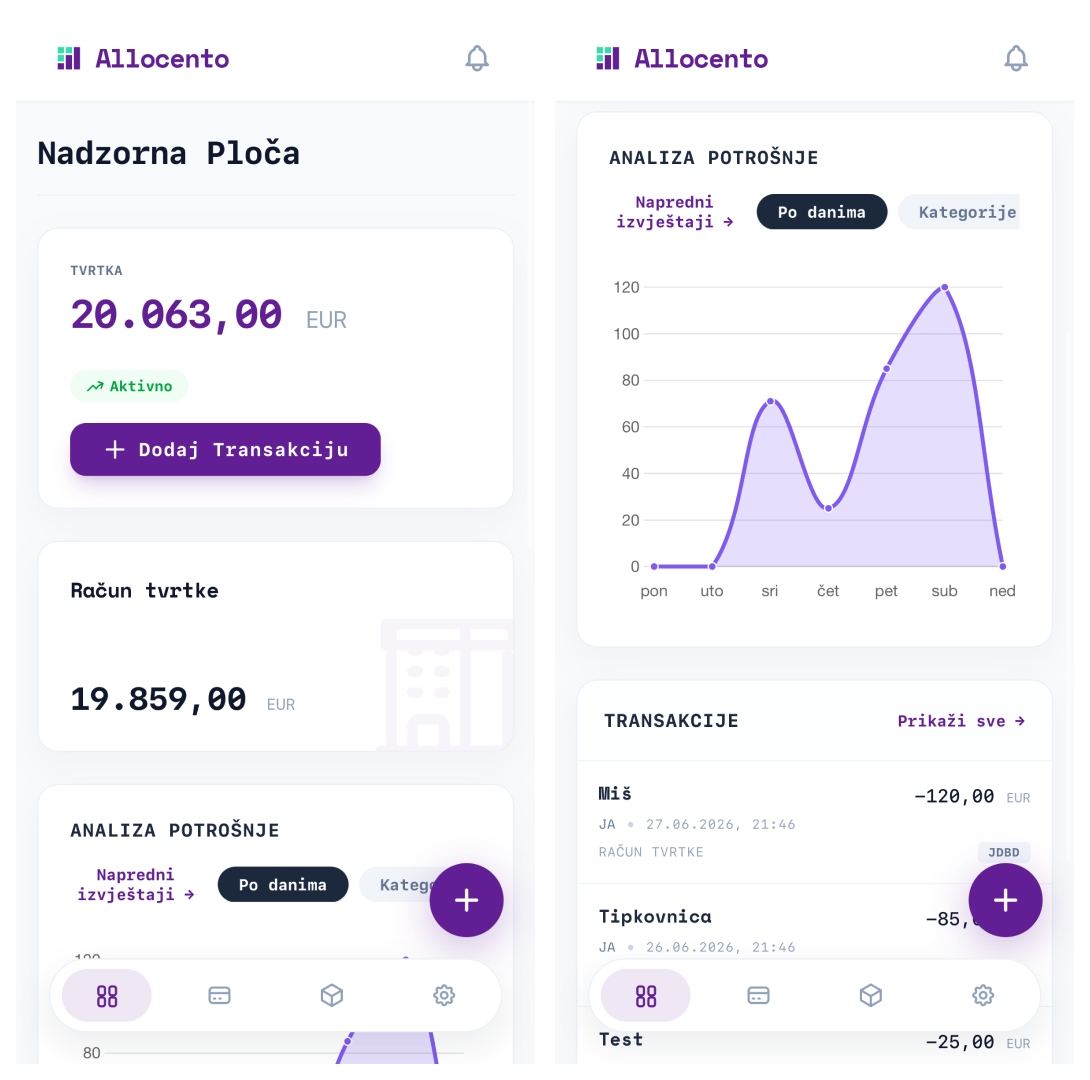
\includegraphics[width=0.9\textwidth]{assets/dashboard.png}
			\caption{Glavna nadzorna ploča sustava Allocento}
			\label{fig:dashboard}
		\end{figure}

		Za detaljniju analizu razvijena je stranica za financijske izvještaje. Korisnik može filtrirati transakcije prema vremenskom razdoblju (npr. tekući mjesec, zadnjih 30 dana, zadnja godina ili prilagođeni raspon), odabranim računima/projektima te kategorijama. 
		
		Izvještaj generira detaljnu tablicu svih stavki i agregirane grafičke prikaze. Korisnik može izvesti generirani financijski izvještaj u PDF formatu klikom na gumb "Izvezi u PDF". Izvoz se provodi u potpunosti na klijentskoj strani pomoću knjižnice za generiranje PDF dokumenata, stvarajući čist i strukturiran dokument spreman za ispis ili slanje klijentima. Sučelje izvještaja i PDF izvoz prikazani su na slici \ref{fig:reports}.

		\begin{figure}[h!]
			\centering
			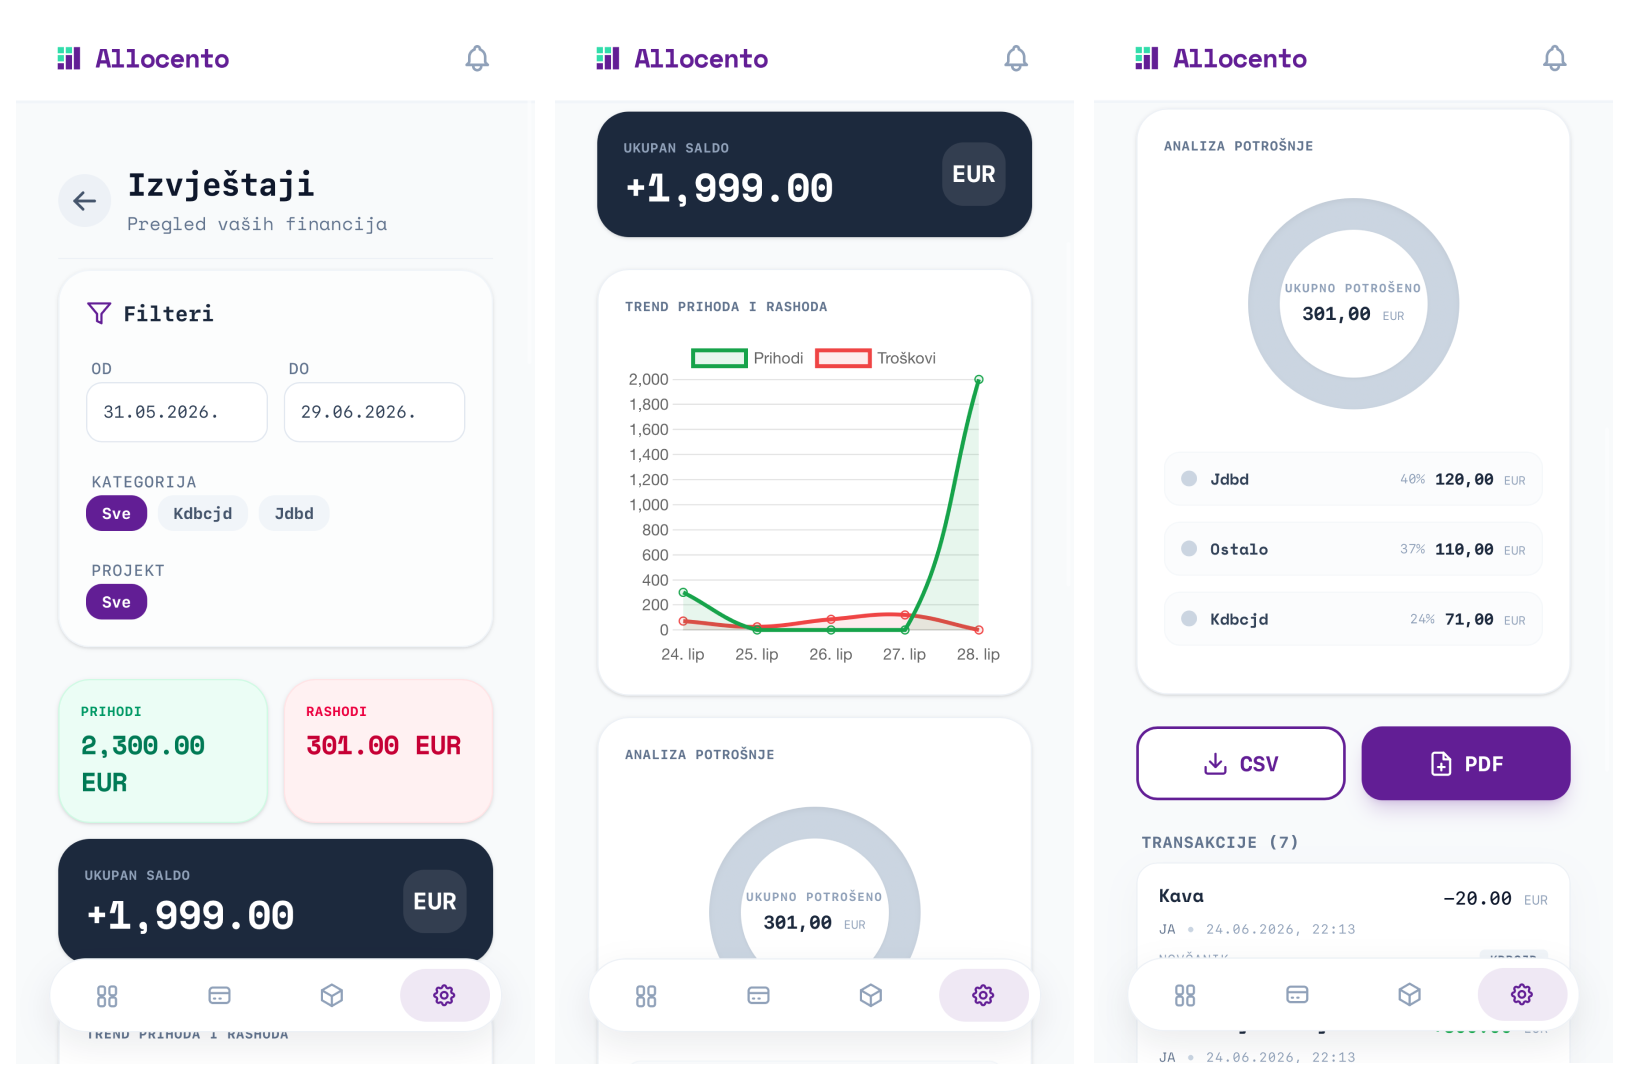
\includegraphics[width=0.85\textwidth]{assets/reports.png}
			\caption{Filtriranje financijskih izvještaja i izvoz u PDF format}
			\label{fig:reports}
		\end{figure}

		\subsection{Prikaz rada sustava u izvanmrežnom načinu rada}
		Ključna prednost Allocento progresivne web aplikacije je sposobnost rada bez internetske veze. Kada klijent izgubi mrežnu vezu, aplikacija ne prekida rad niti prikazuje standardnu pogrešku preglednika o nedostupnosti mreže, već se ponaša na sljedeći način:
		\begin{itemize}
			\item \textbf{Offline indikator:} U zaglavlju aplikacije pokraj logotipa pojavljuje se uočljiva narančasta značka s natpisom "Izvanmrežno".
			
			\item \textbf{Ograničenje sinkronizacijskih akcija:} Izbornik za promjenu radnog prostora se privremeno zaključava ili se prikazuju samo predmemorirani podaci, jer prelazak u novi radni prostor zahtijeva dohvaćanje podataka s poslužitelja.
			
			\item \textbf{Unos transakcije u izvanmrežnom načinu rada:} Korisnik može nesmetano otvoriti formu za dodavanje transakcije, odabrati račun, iznos i kategoriju (koji su učitani iz lokalne IndexedDB baze) te kliknuti "Spremi".
			
			\item \textbf{Prikaz u povijesti:} Transakcija se odmah iscrtava na popisu transakcija i utječe na ukupni saldo prikazan na ekranu, ali je vizualno označena malom ikonom sata ili oblaka koja označava da zapis čeka sinkronizaciju (engl. \textit{pending sync}).
		\end{itemize}
		Prikaz sučelja u izvanmrežnom načinu rada s vidljivim offline indikatorom i transakcijom na čekanju prikazan je na slici \ref{fig:offline-state}.
 
		\begin{figure}[h!]
			\centering
			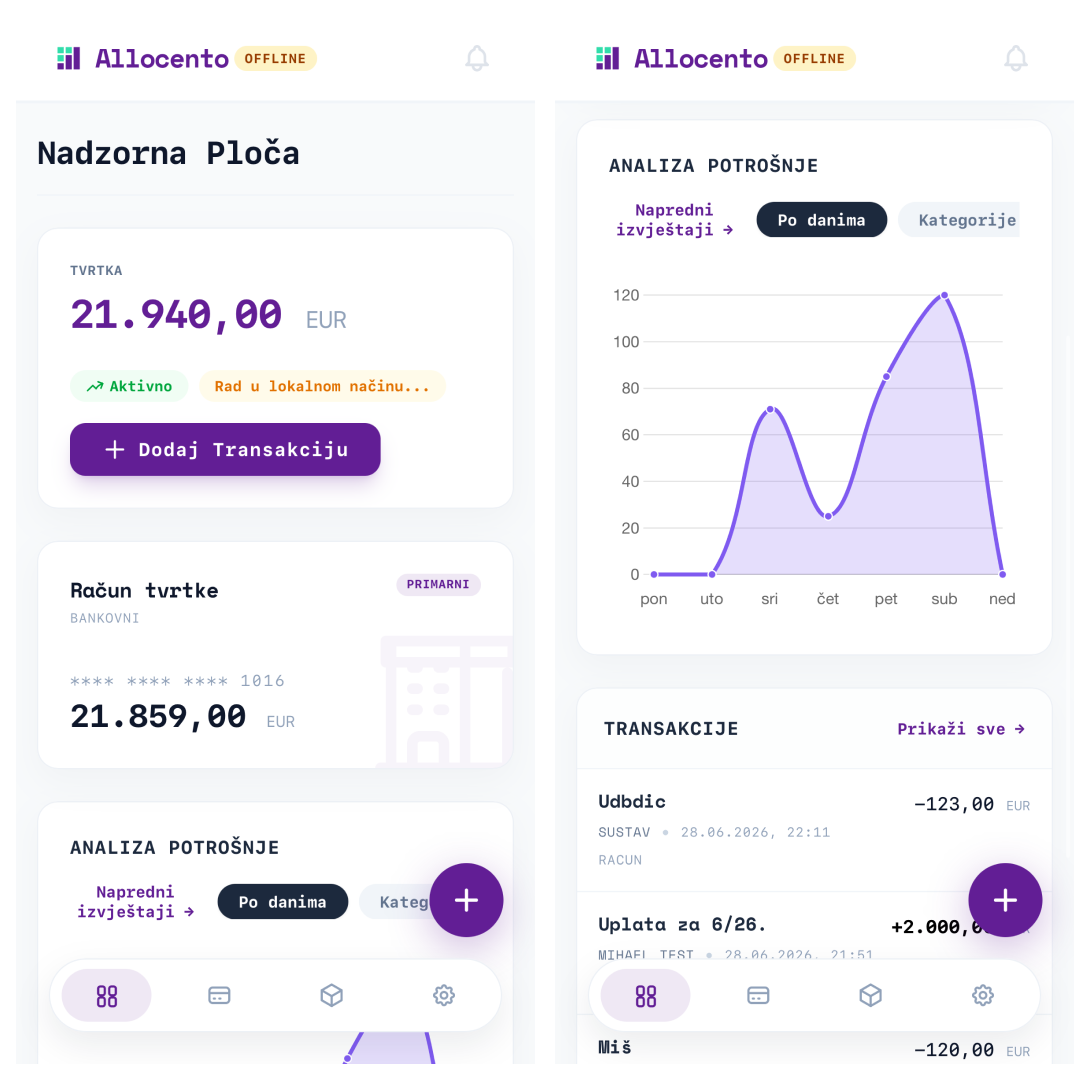
\includegraphics[width=0.85\textwidth]{assets/offline_state.png}
			\caption{Izgled sučelja i unos transakcije u izvanmrežnom načinu rada}
			\label{fig:offline-state}
		\end{figure}
 
		U trenutku kada se mrežna veza vrati, sustav automatski pokreće proces sinkronizacije:
		\begin{itemize}
			\item Značka "Izvanmrežno" u zaglavlju nestaje čim se uspostavi veza, označavajući povratak u mrežni rad.
			
			\item Klijent šalje skupni paket (Bulk Sync) na poslužitelj. Nakon uspješne obrade na poslužitelju, klijent prima stvarni ID transakcije i zamjenjuje privremeni negativni ID u IndexedDB-u.
			
			\item Ikona sata ("pending sync") pokraj transakcije nestaje, označavajući da je podatak uspješno sinkroniziran s glavnom PostgreSQL bazom podataka.
			
			\item Korisniku se isporučuje Web Push obavijest koja potvrđuje uspješnu sinkronizaciju svih offline unosa, čak i ako je u tom trenutku minimizirao aplikaciju.
		\end{itemize}
		Prikaz uspješne sinkronizacije i primljene push obavijesti prikazan je na slici \ref{fig:sync-notification}.

		\begin{figure}[h!]
			\centering
			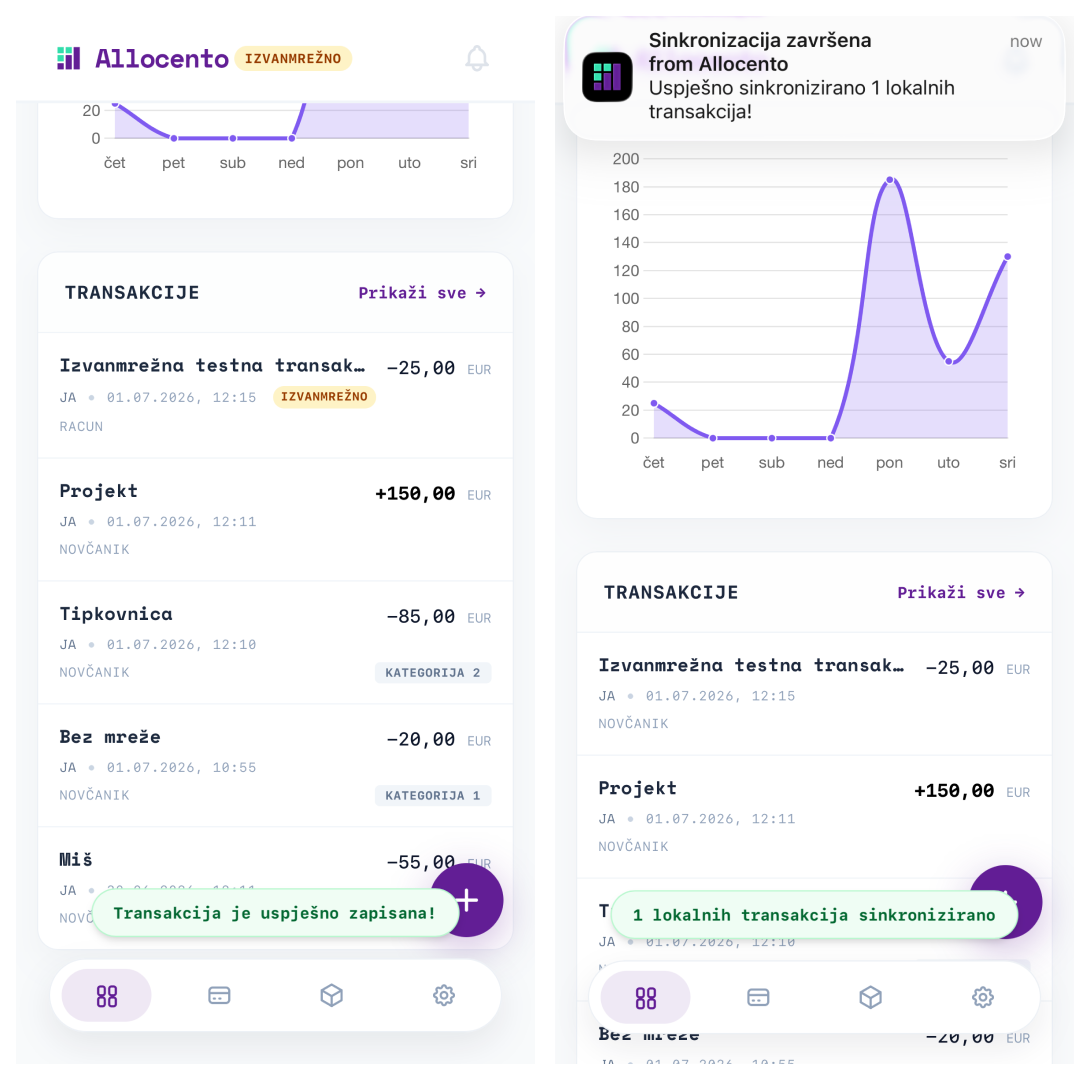
\includegraphics[width=0.8\textwidth]{assets/sync_notification.png}
			\caption{Prikaz obavijesti nakon uspješne sinkronizacije podataka}
			\label{fig:sync-notification}
		\end{figure}
	
	\newpage
	\section{ZAKLJUČAK I BUDUĆI RAD}
		U ovom diplomskom radu uspješno je osmišljen, dizajniran i implementiran sustav "Allocento" - progresivna web aplikacija (PWA) za napredno upravljanje financijskim tokovima, namijenjena pojedincima, timovima i manjim poduzećima. Razvoj sustava uspješno je odgovorio na ključne izazove suvremenih web aplikacija: osiguravanje visoke reaktivnosti korisničkog sučelja, podršku za timsku kolaboraciju uz strogu izolaciju radnih prostora te kontinuitet rada u uvjetima nestabilne internetske veze.

		Odabrani tehnološki stog pokazao se iznimno sinergijskim. Pozadinski dio temeljen na radnom okviru Laravel (PHP) omogućio je brz i siguran razvoj REST API-ja, robusnu validaciju podataka i jednostavnu integraciju Web Push protokola. Klijentski dio razvijen u radnom okviru Angular 17+ iskoristio je prednosti samostalnih komponenti za modularnost i lijeno učitavanje, dok je primjena Angular Signala uvela finu i preciznu reaktivnost, eliminirajući potrebu za teškim i složenim bibliotekama za upravljanje stanjem.

		Najveći tehnički doprinos rada leži u ostvarenju izvanmrežnog rada (engl. \textit{offline mode}) i sinkronizacije. Korištenjem IndexedDB-a omotanog u klijentsku servisnu klasu \texttt{LocalDbService} stvoren je klijentski repozitorijski sloj koji presreće mrežne zahtjeve i omogućuje neprekidno izvođenje CRUD operacija. Generiranjem privremenih negativnih primarnih ključeva i njihovim dodavanjem u lokalni red čekanja ostvareno je trenutačno ažuriranje sučelja. Kada uređaj ponovno uspostavi vezu, osmišljeni algoritam za skupnu sinkronizaciju (Bulk Sync) u jednom HTTP zahtjevu šalje sve offline promjene na poslužitelj, gdje se one unutar jedne SQL transakcije obrađuju i mapiraju na stvarne ID-jeve iz PostgreSQL baze podataka. Time je zajamčena konzistentnost podataka bez opterećivanja mreže višestrukim pojedinačnim API pozivima.

		Uspostavljeni CI/CD cjevovod preko platforme GitHub Actions automatizirao je proces izgradnje i isporuke na produkcijski poslužitelj, čime su skraćeni ciklusi razvoja i eliminirane ljudske pogreške pri implementaciji.

		Iako sustav Allocento u trenutačnom stanju predstavlja potpuno funkcionalnu aplikaciju spremnu za rad, postoji nekoliko otvorenih smjernica za budući rad i nadogradnju:
		\begin{enumerate}
			\item \textbf{Korisničko sučelje za spajanje kategorija:} Iako backend sustava u potpunosti podržava spajanje kategorija transakcija (prenoseći sve povezane transakcije i predloške te brišući staru kategoriju unutar sigurne SQL transakcije), potrebno je razviti intuitivnu formu u klijentskom sučelju koja će korisnicima olakšati ovu operaciju pri reorganizaciji financijskih izvještaja.
			
			\item \textbf{Sučelje za predloške transakcija:} Implementacija vizualnog editora za upravljanje predlošcima transakcija koje se ponavljaju (engl. \textit{RecurringTemplate}), omogućujući korisnicima lakše definiranje periodičkih troškova (npr. mjesečni najam, pretplate).
			
			\item \textbf{Automatsko prepoznavanje računa (OCR):} Integracija tehnologija računalnog vida i optičkog prepoznavanja znakova (engl. \textit{OCR}), čime bi se korisnicima omogućilo jednostavno fotografiranje papirnatih računa na mobilnom uređaju, nakon čega bi sustav automatski izdvojio iznos, datum i naziv trgovca te ispunio formu za transakciju.
			
			\item \textbf{Integracija s otvorenim bankarstvom (PSD2):} Povezivanje aplikacije s API-jevima komercijalnih banaka putem PSD2 protokola. To bi omogućilo automatski uvoz i sinkronizaciju transakcija iz stvarnih bankovnih računa korisnika u radne prostore Allocenta.
			
			\item \textbf{Prediktivna analitika i strojno učenje:} Razvoj naprednih analitičkih modela koji na temelju povijesnih financijskih podataka mogu predvidjeti buduću potrošnju i upozoriti korisnike na potencijalne rizike prekoračenja proračuna u nadolazećim mjesecima.
		\end{enumerate}
	
	\newpage
	\bibliographystyle{unsrt}
	\bibliography{bibtex_baza}
	
	
	\newpage
	\section*{SAŽETAK}
	\addcontentsline{toc}{section}{Sažetak}
	Tema ovog diplomskog rada je razvoj i implementacija sustava "Allocento" - progresivne web aplikacije (PWA) za upravljanje osobnim i timskim financijskim tokovima. Glavni cilj rada je stvoriti rješenje koje korisnicima pruža reaktivno, sigurno i moderno sučelje s podrškom za rad u uvjetima nestabilne internetske veze te timsku kolaboraciju.
	
	Pozadinski dio sustava realiziran je pomoću programskog jezika PHP i razvojnog okvira Laravel, koji služi kao REST API i osigurava autentifikaciju (Laravel Sanctum), autorizaciju, provjeru prava pristupa kroz prilagođeni middleware za izolaciju radnih prostora te integraciju Web Push protokola. Klijentski dio aplikacije izgrađen je pomoću programskog jezika TypeScript i razvojnog okvira Angular, gdje se za reaktivno upravljanje stanjima i optimalno iscrtavanje sučelja koriste Angular Signali.
	
	Poseban naglasak stavljen je na offline rad i sinkronizaciju podataka. Korištenjem IndexedDB lokalne baze podataka i prilagođene klijentske klase \texttt{LocalDbService} klijent bilježi sve operacije kada je uređaj izvan mreže. Nakon ponovnog spajanja na internet, razvijeni algoritam za skupnu sinkronizaciju (Bulk Sync) u jednom zahtjevu sinkronizira sve promjene s poslužiteljem unutar jedne SQL transakcije. CI/CD cjevovod preko platforme GitHub Actions automatizira postupak isporuke aplikacije na produkcijski poslužitelj.
	
	\bigskip
	\noindent\textbf{Ključne riječi:} progresivna web aplikacija, Angular, Laravel, IndexedDB, sinkronizacija podataka, Web Push obavijesti, upravljanje financijama.
	
	
	\newpage
	\section*{Abstract}
	\addcontentsline{toc}{section}{Abstract}
	The subject of this master's thesis is the development and implementation of "Allocento" - a progressive web application (PWA) for personal and team financial management. The main objective of the thesis is to create a solution that provides users with a reactive, secure, and modern interface, supporting work under unstable internet connection conditions and facilitating team collaboration.
	
	The backend part of the system is realized using PHP and the Laravel framework, which serves as a REST API and ensures authentication (Laravel Sanctum), authorization, access control check through custom middleware for workspace isolation, and integration of the Web Push protocol. The client-side application is built using TypeScript and the Angular framework, utilizing Angular Signals for reactive state management and optimal UI rendering.
	
	Special emphasis is placed on offline functionality and data synchronization. By using IndexedDB local storage and a custom client service wrapper, the client records all operations when the device is offline. Upon reconnecting, the developed bulk synchronization algorithm synchronizes all changes with the server in a single HTTP request within a single database transaction. Finally, a Base CI/CD pipeline via GitHub Actions automates the deployment process of the application to the production server.
	
	\bigskip
	\noindent\textbf{Keywords:} progressive web application, Angular, Laravel, IndexedDB, data synchronization, Web Push notifications, financial management.
	
	
	\newpage
	\section*{Životopis}
	\addcontentsline{toc}{section}{Životopis}
	
	
	\newpage
	\section*{Prilozi}
	\addcontentsline{toc}{section}{Prilozi}
	
	\end{document}